\documentclass[./main.tex]{subfiles}

     
\begin{document}

\section{Contig classification ~\label{sec:appendix_contig_classification}}

In order to have a better understanding of the contig graph produced by a given assembler, we wish to filter out contigs that are not of chromosomal origin. %
We compare each contig against the \emph{nr} database using Megablast (Morgulis et al., 2008), and classify a contig as chromosomal if its length is greater than 1 Mb, or is such that 80\% of the first 50 Megablast hits map to a complete bacterial genome. %
We use the same second criterion to classify whether a contig is of plasmid origin, regardless of its size. %
Remaining unclassified contigs are classified as of undefined origin. %
In addition, we flag as \emph{containment} contigs those which map (using \minimap) over at least 75\% of their length to another contig.%




\section{On whether \canu contig fragmentation can be solved using \miniasm contigs \label{sec:appendix:gap_comparison}}


To check if \miniasm contigs could possibly enable to order and fill gaps between \canu contigs, we performed an assembly using the \minimap and \miniasm pipeline using both the \canu contigs and the \miniasm contigs as input (to be clear: no reads were used as input to this assembly, only two contig sets). To allow \minimap to find shorter matches, mapping of \miniasm contigs against \canu contigs was performed with the following parameters: \texttt{-x map-pb -m 25 -n 2}. To avoid \miniasm filtering overlaps,  we ran it with the following parameters: \texttt{-1 -2 -s 1000 -c 0}.

We ran this pipeline on all datasets, and counted the number of times that a \miniasm contig overlaps with two \canu contigs. We also counted the number of contigs generated by \miniasm using the overlap created at the previous step. Results are summarized in Supplementary Table \ref{tab:appendix:gap_comparison}.


\begin{table}[!htbp]
    \centering
    \begin{tabular}{l|rr|rr}
    \hline
        & \multicolumn{2}{r|}{number of genomic contig} & number of \miniasm    & number of merged contigs \\
        &  &                                            & contigs that overlap  & contigs from  \\ 
NCTC ID & \canu &  \miniasm                             & two \canu contigs & \miniasm/\canu overlaps \\ \hline
NCTC10006	&	3	&	7	&	0	&	0	\\
NCTC10332	&	12	&	22	&	1	&	0	\\
NCTC10444	&	7	&	5	&	0	&	0	\\
NCTC10702	&	3	&	2	&	0	&	0	\\
NCTC10766	&	13	&	7	&	1	&	0	\\
NCTC10794	&	7	&	5	&	0	&	0	\\
NCTC10988	&	10	&	9	&	0	&	0	\\
NCTC11126	&	7	&	15	&	5	&	0	\\
NCTC11343	&	12	&	10	&	2	&	1	\\
NCTC11360	&	26	&	25	&	1	&	0	\\
NCTC11435	&	8	&	6	&	2	&	0	\\
NCTC11800	&	7	&	3	&	1	&	0	\\
NCTC11872	&	7	&	13	&	3	&	0	\\
NCTC12123	&	5	&	3	&	2	&	0	\\
NCTC12126	&	13	&	15	&	4	&	0	\\
NCTC12131	&	16	&	77	&	3	&	0	\\
NCTC12132	&	2	&	4	&	1	&	0	\\
NCTC12146	&	3	&	1	&	0	&	0	\\
NCTC12694	&	21	&	123	&	1	&	0	\\
NCTC12841	&	16	&	1	&	0	&	0	\\
NCTC12993	&	5	&	2	&	0	&	0	\\
NCTC12998	&	3	&	4	&	0	&	0	\\
NCTC13095	&	3	&	2	&	0	&	0	\\
NCTC13125	&	6	&	7	&	0	&	0	\\
NCTC13348	&	25	&	17	&	3	&	1	\\
NCTC13463	&	5	&	4	&	1	&	0	\\
NCTC13543	&	3	&	3	&	0	&	0	\\
NCTC4672	&	68	&	16	&	5	&	1	\\
NCTC5050	&	4	&	4	&	0	&	0	\\
NCTC5053	&	8	&	11	&	2	&	1	\\
NCTC5055	&	143	&	20	&	0	&	0	\\
NCTC7922	&	13	&	9	&	4	&	1	\\
NCTC8179	&	15	&	15	&	1	&	0	\\
NCTC8500	&	3	&	1	&	0	&	1	\\
NCTC8684	&	5	&	2	&	0	&	0	\\
NCTC9075	&	7	&	3	&	2	&	0	\\
NCTC9078	&	4	&	2	&	0	&	0	\\
NCTC9098	&	8	&	6	&	3	&	0	\\
NCTC9111	&	9	&	13	&	0	&	0	\\
NCTC9112	&	7	&	15	&	10	&	0	\\
NCTC9184	&	141	&	17	&	0	&	0	\\
NCTC9645	&	31	&	76	&	9	&	3	\\
NCTC9646	&	8	&	9	&	3	&	1	\\
NCTC9695	&	2	&	1	&	0	&	0	\\
 \hline
    \end{tabular}
    \caption{
    The pipeline described section \ref{sec:appendix:gap_comparison} found more than one overlap between \canu contigs with \miniasm contig for 24 over 45 datasets. When these overlaps are re-assembled  using \miniasm, one or more merged contigs are produced in only 8 out of 45 datasets.
    }
    \label{tab:appendix:gap_comparison}
\end{table}


\newpage

\section{Assembly summary ~\label{sec:appendix_assembly_summary}}

Tables ~\ref{tb:appendix:assembly_resume} and~\ref{tb:appendix:path_search_result} report our complete results for the 45 NCTC datasets.
\begin{table}[!htbp]
\small
\begin{tabular}{l|l|r|rrr|l|rrr|rrr}
\hline
           & & & \multicolumn{3}{c|}{NCTC contigs} & \hinge  &
                                                              \multicolumn{3}{c|}{\canu contigs} & \multicolumn{3}{c}{\miniasm contigs} \\
NCTC ID    & species     &  cov & chr &  pld & und & status & chr & pld & und & chr & pld & und \\\hline
    \csvreader[head to column names]{supplemental/knot/summary_assembly.csv}{}%
    {\\\nctcid	& \textit{\species} & \coverage & \nctccontigchr & \nctccontigpld & \nctccontigund & \hingestatus & \canucontigschr & \canucontigspld & \canucontigsund & \miniasmcontigschr & \miniasmcontigspld & \miniasmcontigsund}%
    \\\hline
\end{tabular}
\caption{Datasets from the NCTC project chosen for analysis (the last row corresponds to our simulated dataset). For each sample, the coverage (cov) is given as well as the number of contigs and their assignment; chr: number of chromosomal contigs, pld: number of plasmid contigs, und: number of other contigs. For two datasets (NCTC12841 and NCTC9646) the NCTC project does not yet provide an assembly ("Pending"). For \canu and \miniasm, a classification similar to the one of NCTC is given (see text). We reported \hinge classification; FALC: Finished assembly (lacking circularization), FA: Finished assembly, MA: Mis-assembly, MA$^*$: labeled as misassembled but actually correctly solved as 2 chromosomes, FCA: Finished circular assembly, MAF: Mis-assembly/Fragmented, FAMT: Finished assembly with multiple traversals.}
\label{tb:appendix:assembly_resume}
\end{table}

\begin{table}[!htbp]
\footnotesize

\begin{tabular}{l|cc|c|cc|cccc}
\hline
 & \multicolumn{2}{c|}{\canu} & & \multicolumn{5}{c}{Edges in the AAG} \\
NCTC ID & contigs & dead-ends & dead-ends & total AAG & theoretical & distant & \multicolumn{3}{c}{adjacency edges}\\
 & & & with adj. & & max. &  edges & total & single & multiple \\
 & & & edge      & & edges &        &       &        & \\
 \hline
     \csvreader[head to column names]{supplemental/knot/path_search_resume.csv}{}%
    {\\\NCTCID & \contigcanu & \deadend & \deadendsolved & \allpath & \theoricalpath & \discard & \good & \goodnorepeat & \goodrepeat}%
    \\\hline
\end{tabular}


\caption{Assembly graph statistics for a selection of 45 fragmented assemblies from the NCTC project.  \canu assembly graph statistics: number of contigs, number of dead-end extremities. AAG statistics: theoretical maximal number number of edges. Note that for some of the most fragmented datasets (e.g. NCTC9184), none of the contigs pass the 100 Kbp length threshold, hence the AAG is empty.} 
\label{tb:appendix:path_search_result}
\end{table}


\begin{table}[]
    \centering
    \small
    \begin{tabular}{l c}
        Mean number of& \\
        \hline
         \miniasm contigs & 5.8 \\
         \hline
         Edges in AAG & 85.1\\
         Theoretical max. edges in AAG & 94.4 \\
         Distant edges & 83.12 \\
         All adjacency edges & 1.98 \\
         Single adjacency edges & 1.51 \\
         Multiple adjacency edges & 0.46 \\
         \hline
         Dead-ends in \miniasm contigs &  11.61 \\
         Dead-ends in AAG, adjacency edges & 7.95 \\ % 1.2 en non repeat
        \hline
    \end{tabular}
    \caption{Average statistics of augmented assembly graphs using a SG built from \minimap overlaps on \miniasm contigs across the 37 NCTC datasets with two or more contigs, after size and classification filters.
    All rows are as per definitions in Section~\ref{sec:aag}. 'Theoretical max. edges': number of possible edges in each AAG. 'Dead-ends in AAG, adjacency edges': number of dead-ends in the AAG when only adjacency edges are considered, i.e. distant edges are deleted.}
    \label{tab:appendix:path_search_resume_miniasm}
\end{table}


\begin{table}[!htbp]
\footnotesize

\begin{tabular}{l|cc|c|cc|cccc}
\hline
 & \multicolumn{2}{c|}{\miniasm} & & \multicolumn{5}{c}{Edges in the AAG} \\
NCTC ID & contigs & dead-ends & dead-ends & total AAG & theoretical & distant & \multicolumn{3}{c}{adjacency edges}\\
 & & & with adj. & & max. &  edges & total & single & multiple \\
 & & & edge      & & edges &        &       &        & \\
 \hline
     \csvreader[head to column names]{supplemental/knot/path_search_resume_miniasm.csv}{}%
    {\\\NCTCID & \contigcanu & \deadend & \deadendsolved & \allpath & \theoricalpath & \discard & \good & \goodnorepeat & \goodrepeat}%
    \\\hline
\end{tabular}


\caption{Assembly graph statistics for a selection of 45 fragmented assemblies from the NCTC project. \miniasm assembly graph statistics: number of contigs, number of dead-end extremities. AAG statistics: theoretical maximal number number of edges. Note that for some of the most fragmented datasets (e.g. NCTC9184), none of the contigs pass the 100 Kbp length threshold, hence the AAG is empty. '*'  denotes dataset for which the result is not available.} 
\label{tb:appendix:path_search_result_miniasm}
\end{table}

\newpage

\section{}

\begin{figure}[!htbp]
    \centering
    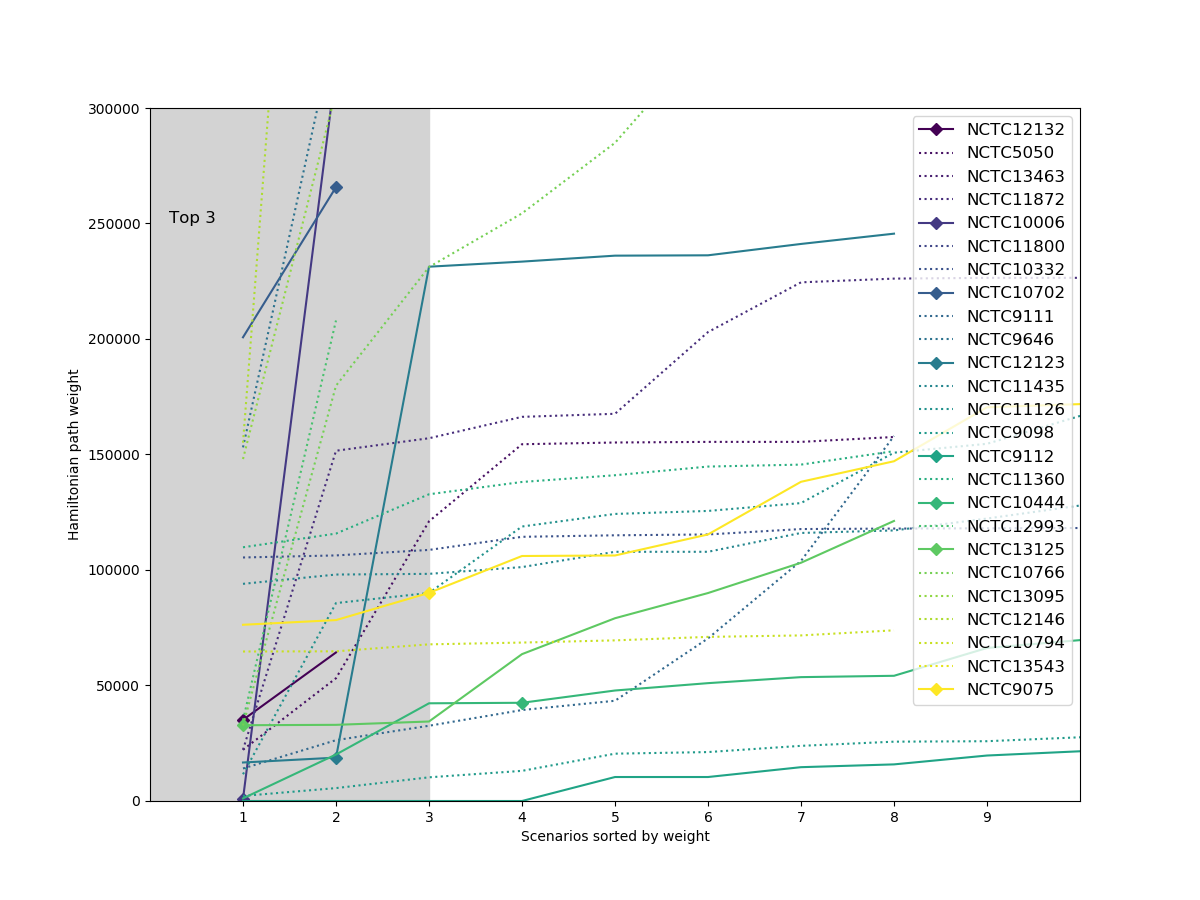
\includegraphics[width=0.6\textwidth]{supplemental/knot/hamilton_path.png}
    \caption{Weights of scenarios in AAGs. Each curve correspond to the sorted
list of Hamiltonian cycles, sorted by weight. If a ground truth is known,
a diamond symbol marks the correct assembly scenario}
    \label{fig:appendix:hamilton_path}
\end{figure}


\newpage

\twocolumn
\section{Contigs length and classification}
\subsection*{Canu}
{\scriptsize
\bottomcaption{Canu contigs classification per NCTC dataset. Total length of chromosomal contigs is given.\label{tb:appendix:canu_NCTC_contigs}}
\tablefirsthead{%
Dataset & Contig name & Classification & Length \\%
\hline \hline}
\begin{supertabular}{llcr}
%Dataset & Contig name & Assignation & Length \\
%\hline \hline
NCTC10006 & tig00000055 & chromosomal & 635691 \\
          & tig00001802 & chromosomal & 4649423 \\
          & tig00001803 & chromosomal & 11996 \\
 & \multicolumn{2}{r}{\cellcolor{black!25} total chromosomal length}  & \cellcolor{black!25} 5297110 \\
\cline{2-4}
\hline \hline
NCTC10332 & tig00000001 & chromosomal & 3474338 \\
          & tig00000002 & chromosomal & 30165 \\
          & tig00000049 & chromosomal & 477163 \\
          & tig00000076 & chromosomal & 781581 \\
          & tig00000121 & chromosomal & 2609 \\
          & tig00000123 & chromosomal & 2461 \\
          & tig00000125 & chromosomal & 2452 \\
          & tig00009835 & chromosomal & 2395 \\
          & tig00009836 & chromosomal & 1564849 \\
          & tig00009837 & chromosomal & 11088 \\
          & tig00009838 & chromosomal & 2340 \\
          & tig00009839 & chromosomal & 2302 \\
 & \multicolumn{2}{r}{\cellcolor{black!25} total chromosomal length}  & \cellcolor{black!25} 6353743 \\
\cline{2-4}
\hline \hline
NCTC10444 & tig00000085 & chromosomal & 16691 \\
          & tig00000105 & chromosomal & 989155 \\
          & tig00000671 & chromosomal & 2391267 \\
          & tig00000672 & chromosomal & 14372 \\
          & tig00000673 & chromosomal & 1333749 \\
          & tig00000674 & chromosomal & 9774 \\
          & tig00000675 & chromosomal & 603044 \\
 & \multicolumn{2}{r}{\cellcolor{black!25} total chromosomal length}  & \cellcolor{black!25} 5358052 \\
\cline{2-4}
\hline \hline
NCTC10702 & tig00000001 & chromosomal & 1882575 \\
          & tig00000002 & chromosomal & 1048854 \\
          & tig00000080 & chromosomal & 70302 \\
 & \multicolumn{2}{r}{\cellcolor{black!25} total chromosomal length}  & \cellcolor{black!25} 3001731 \\
\cline{2-4}
          & tig00000200 & plasmidic & 49994 \\
          & tig00001328 & plasmidic & 28893 \\
          & tig00001329 & plasmidic & 7575 \\
\cline{2-4}
          & tig00000084 & undefined & 30012 \\
          & tig00000087 & undefined & 2442 \\
          & tig00000199 & undefined & 20259 \\
\cline{2-4}
\hline \hline
NCTC10766 & tig00000009 & chromosomal & 35058 \\
          & tig00000021 & chromosomal & 331047 \\
          & tig00001907 & chromosomal & 4740 \\
          & tig00001908 & chromosomal & 3602512 \\
          & tig00001909 & chromosomal & 15279 \\
          & tig00001910 & chromosomal & 700851 \\
          & tig00001911 & chromosomal & 14965 \\
          & tig00001912 & chromosomal & 10378 \\
          & tig00001913 & chromosomal & 20674 \\
          & tig00001915 & chromosomal & 10586 \\
          & tig00001916 & chromosomal & 9467 \\
          & tig00001921 & chromosomal & 7453 \\
          & tig00001922 & chromosomal & 710378 \\
 & \multicolumn{2}{r}{\cellcolor{black!25} total chromosomal length}  & \cellcolor{black!25} 5473388 \\
\cline{2-4}
          & tig00000032 & plasmidic & 91068 \\
          & tig00000038 & plasmidic & 6441 \\
          & tig00000057 & plasmidic & 49757 \\
          & tig00001917 & plasmidic & 30098 \\
          & tig00001918 & plasmidic & 12494 \\
          & tig00001919 & plasmidic & 8557 \\
          & tig00001920 & plasmidic & 22116 \\
\cline{2-4}
          & tig00000035 & undefined & 7262 \\
          & tig00000036 & undefined & 3368 \\
\cline{2-4}
\hline \hline
NCTC10794 & tig00000006 & chromosomal & 54912 \\
          & tig00000027 & chromosomal & 3322 \\
          & tig00000081 & chromosomal & 92448 \\
          & tig00000108 & chromosomal & 3328 \\
          & tig00000189 & chromosomal & 480759 \\
          & tig00000190 & chromosomal & 290320 \\
          & tig00004951 & chromosomal & 591102 \\
 & \multicolumn{2}{r}{\cellcolor{black!25} total chromosomal length}  & \cellcolor{black!25} 1516191 \\
\cline{2-4}
          & tig00000003 & undefined & 186664 \\
          & tig00000014 & undefined & 105799 \\
          & tig00000039 & undefined & 180586 \\
          & tig00000040 & undefined & 18002 \\
          & tig00000042 & undefined & 42405 \\
          & tig00000047 & undefined & 41214 \\
          & tig00000067 & undefined & 3608 \\
          & tig00000072 & undefined & 3493 \\
          & tig00000098 & undefined & 3650 \\
          & tig00000100 & undefined & 3534 \\
          & tig00000102 & undefined & 3498 \\
          & tig00000110 & undefined & 1327 \\
          & tig00000114 & undefined & 3322 \\
          & tig00000116 & undefined & 3800 \\
          & tig00000187 & undefined & 16904 \\
          & tig00000188 & undefined & 12596 \\
          & tig00000191 & undefined & 12836 \\
          & tig00000192 & undefined & 12673 \\
          & tig00004950 & undefined & 4641 \\
          & tig00004952 & undefined & 105999 \\
          & tig00004953 & undefined & 11722 \\
          & tig00004954 & undefined & 6412 \\
          & tig00004955 & undefined & 9623 \\
\cline{2-4}
          & tig00000096 & none & 5730 \\
          & tig00000112 & none & 1434 \\
          & tig00000186 & none & 5922 \\
\cline{2-4}
\hline \hline
NCTC10988 & tig00000006 & chromosomal & 25636 \\
          & tig00000279 & chromosomal & 3040963 \\
          & tig00000896 & chromosomal & 22144 \\
          & tig00000897 & chromosomal & 19058 \\
          & tig00000898 & chromosomal & 14604 \\
          & tig00000899 & chromosomal & 14371 \\
          & tig00000900 & chromosomal & 13453 \\
          & tig00000901 & chromosomal & 19223 \\
          & tig00000902 & chromosomal & 14801 \\
          & tig00000903 & chromosomal & 17641 \\
 & \multicolumn{2}{r}{\cellcolor{black!25} total chromosomal length}  & \cellcolor{black!25} 3201894 \\
\cline{2-4}
          & tig00000088 & undefined & 4456 \\
          & tig00000105 & undefined & 36448 \\
\cline{2-4}
\hline \hline
NCTC11126 & tig00000037 & chromosomal & 577906 \\
          & tig00000074 & chromosomal & 666697 \\
          & tig00000192 & chromosomal & 1514971 \\
          & tig00000193 & chromosomal & 6302 \\
          & tig00000194 & chromosomal & 2066502 \\
          & tig00003788 & chromosomal & 8944 \\
          & tig00003789 & chromosomal & 46666 \\
 & \multicolumn{2}{r}{\cellcolor{black!25} total chromosomal length}  & \cellcolor{black!25} 4887988 \\
\cline{2-4}
\hline \hline
NCTC11343 & tig00000004 & chromosomal & 11272 \\
          & tig00000067 & chromosomal & 117209 \\
          & tig00000083 & chromosomal & 258828 \\
          & tig00000095 & chromosomal & 5614 \\
          & tig00000272 & chromosomal & 249754 \\
          & tig00000291 & chromosomal & 226277 \\
          & tig00000726 & chromosomal & 2208641 \\
          & tig00005693 & chromosomal & 12001 \\
          & tig00005694 & chromosomal & 876928 \\
          & tig00005696 & chromosomal & 3878 \\
          & tig00005698 & chromosomal & 8934 \\
          & tig00005699 & chromosomal & 214339 \\
 & \multicolumn{2}{r}{\cellcolor{black!25} total chromosomal length}  & \cellcolor{black!25} 4193675 \\
\cline{2-4}
          & tig00000047 & undefined & 470559 \\
          & tig00000158 & undefined & 3400 \\
          & tig00000261 & undefined & 3105 \\
          & tig00000357 & undefined & 55998 \\
          & tig00000360 & undefined & 46002 \\
          & tig00000381 & undefined & 1809 \\
          & tig00000727 & undefined & 136723 \\
          & tig00000728 & undefined & 6803 \\
          & tig00000729 & undefined & 19083 \\
          & tig00000730 & undefined & 6003 \\
          & tig00005695 & undefined & 783131 \\
          & tig00005697 & undefined & 20459 \\
          & tig00005700 & undefined & 12630 \\
          & tig00005701 & undefined & 4319 \\
          & tig00005702 & undefined & 4350 \\
          & tig00005703 & undefined & 325592 \\
          & tig00005704 & undefined & 8727 \\
\cline{2-4}
\hline \hline
NCTC11360 & tig00000001 & chromosomal & 856759 \\
          & tig00000002 & chromosomal & 167905 \\
          & tig00000023 & chromosomal & 2941 \\
          & tig00000024 & chromosomal & 74373 \\
          & tig00000036 & chromosomal & 2775 \\
          & tig00000039 & chromosomal & 4498 \\
          & tig00000040 & chromosomal & 90923 \\
          & tig00000044 & chromosomal & 93819 \\
          & tig00000059 & chromosomal & 3339 \\
          & tig00000061 & chromosomal & 5726 \\
          & tig00000067 & chromosomal & 69601 \\
          & tig00000084 & chromosomal & 2711 \\
          & tig00000115 & chromosomal & 85300 \\
          & tig00000116 & chromosomal & 6833 \\
          & tig00000117 & chromosomal & 89165 \\
          & tig00000118 & chromosomal & 7948 \\
          & tig00000119 & chromosomal & 73822 \\
          & tig00000121 & chromosomal & 61437 \\
          & tig00000122 & chromosomal & 11175 \\
          & tig00000123 & chromosomal & 7718 \\
          & tig00002040 & chromosomal & 3708 \\
          & tig00002041 & chromosomal & 446407 \\
          & tig00002042 & chromosomal & 2667 \\
          & tig00002043 & chromosomal & 3997 \\
          & tig00002044 & chromosomal & 6676 \\
          & tig00002045 & chromosomal & 6999 \\
 & \multicolumn{2}{r}{\cellcolor{black!25} total chromosomal length}  & \cellcolor{black!25} 2189222 \\
\cline{2-4}
\hline \hline
NCTC11435 & tig00000001 & chromosomal & 1450647 \\
          & tig00000002 & chromosomal & 1627001 \\
          & tig00000267 & chromosomal & 3308 \\
          & tig00001171 & chromosomal & 213960 \\
          & tig00001172 & chromosomal & 11255 \\
          & tig00001173 & chromosomal & 260680 \\
          & tig00001174 & chromosomal & 13563 \\
          & tig00001175 & chromosomal & 871963 \\
 & \multicolumn{2}{r}{\cellcolor{black!25} total chromosomal length}  & \cellcolor{black!25} 4452377 \\
\cline{2-4}
\hline \hline
NCTC11800 & tig00000003 & chromosomal & 2775 \\
          & tig00000100 & chromosomal & 2617 \\
          & tig00000108 & chromosomal & 2163 \\
          & tig00000110 & chromosomal & 2403 \\
          & tig00000228 & chromosomal & 797974 \\
          & tig00000229 & chromosomal & 7782 \\
          & tig00003669 & chromosomal & 3650645 \\
 & \multicolumn{2}{r}{\cellcolor{black!25} total chromosomal length}  & \cellcolor{black!25} 4466359 \\
\cline{2-4}
          & tig00000002 & undefined & 2722 \\
          & tig00000104 & undefined & 2273 \\
          & tig00003670 & undefined & 10818 \\
\cline{2-4}
\hline \hline
NCTC11872 & tig00000016 & chromosomal & 486488 \\
          & tig00000035 & chromosomal & 414114 \\
          & tig00000200 & chromosomal & 305814 \\
          & tig00000201 & chromosomal & 6170 \\
          & tig00000202 & chromosomal & 554139 \\
          & tig00000203 & chromosomal & 6679 \\
          & tig00000204 & chromosomal & 106287 \\
 & \multicolumn{2}{r}{\cellcolor{black!25} total chromosomal length}  & \cellcolor{black!25} 1879691 \\
\cline{2-4}
          & tig00000072 & undefined & 1688 \\
\cline{2-4}
\hline \hline
NCTC12123 & tig00000001 & chromosomal & 2025792 \\
          & tig00000002 & chromosomal & 2402021 \\
          & tig00000009 & chromosomal & 319720 \\
          & tig00001215 & chromosomal & 17954 \\
          & tig00001216 & chromosomal & 19022 \\
 & \multicolumn{2}{r}{\cellcolor{black!25} total chromosomal length}  & \cellcolor{black!25} 4784509 \\
\cline{2-4}
          & tig00000045 & plasmidic & 7248 \\
          & tig00001219 & plasmidic & 14495 \\
          & tig00001220 & plasmidic & 11169 \\
          & tig00001221 & plasmidic & 12838 \\
\cline{2-4}
          & tig00000003 & undefined & 7552 \\
          & tig00000036 & undefined & 2048 \\
          & tig00001217 & undefined & 44732 \\
          & tig00001218 & undefined & 4652 \\
\cline{2-4}
\hline \hline
NCTC12126 & tig00000002 & chromosomal & 2504 \\
          & tig00000003 & chromosomal & 6347 \\
          & tig00000005 & chromosomal & 312284 \\
          & tig00000018 & chromosomal & 697355 \\
          & tig00000041 & chromosomal & 180413 \\
          & tig00000088 & chromosomal & 980155 \\
          & tig00000103 & chromosomal & 2869 \\
          & tig00000144 & chromosomal & 58545 \\
          & tig00000151 & chromosomal & 9045 \\
          & tig00000154 & chromosomal & 4231 \\
          & tig00000255 & chromosomal & 1991519 \\
          & tig00000256 & chromosomal & 3006 \\
          & tig00000257 & chromosomal & 620710 \\
 & \multicolumn{2}{r}{\cellcolor{black!25} total chromosomal length}  & \cellcolor{black!25} 4868983 \\
\cline{2-4}
          & tig00000119 & plasmidic & 168880 \\
\cline{2-4}
\hline \hline
NCTC12131 & tig00000004 & chromosomal & 585202 \\
          & tig00000022 & chromosomal & 2720 \\
          & tig00000052 & chromosomal & 782381 \\
          & tig00000129 & chromosomal & 3215 \\
          & tig00000133 & chromosomal & 2760 \\
          & tig00000260 & chromosomal & 277244 \\
          & tig00000261 & chromosomal & 6991 \\
          & tig00000262 & chromosomal & 654135 \\
          & tig00000263 & chromosomal & 7044 \\
          & tig00000264 & chromosomal & 44446 \\
          & tig00000265 & chromosomal & 6070 \\
          & tig00000266 & chromosomal & 658311 \\
          & tig00000267 & chromosomal & 173281 \\
          & tig00000268 & chromosomal & 6652 \\
          & tig00000269 & chromosomal & 735339 \\
          & tig00000271 & chromosomal & 839355 \\
 & \multicolumn{2}{r}{\cellcolor{black!25} total chromosomal length}  & \cellcolor{black!25} 4785146 \\
\cline{2-4}
          & tig00000272 & undefined & 11590 \\
          & tig00000273 & undefined & 3170 \\
\cline{2-4}
\hline \hline
NCTC12132 & tig00000001 & chromosomal & 2583454 \\
          & tig00000002 & chromosomal & 756442 \\
 & \multicolumn{2}{r}{\cellcolor{black!25} total chromosomal length}  & \cellcolor{black!25} 3339896 \\
\cline{2-4}
          & tig00000004 & undefined & 20873 \\
\cline{2-4}
\hline \hline
NCTC12146 & tig00000001 & chromosomal & 4385596 \\
          & tig00001748 & chromosomal & 15170 \\
          & tig00001749 & chromosomal & 1248170 \\
 & \multicolumn{2}{r}{\cellcolor{black!25} total chromosomal length}  & \cellcolor{black!25} 5648936 \\
\cline{2-4}
\hline \hline
NCTC12694 & tig00000001 & chromosomal & 1305929 \\
          & tig00000004 & chromosomal & 723799 \\
          & tig00000010 & chromosomal & 270213 \\
          & tig00000013 & chromosomal & 244711 \\
          & tig00000015 & chromosomal & 205059 \\
          & tig00000017 & chromosomal & 163002 \\
          & tig00000019 & chromosomal & 200318 \\
          & tig00000021 & chromosomal & 138348 \\
          & tig00000028 & chromosomal & 101438 \\
          & tig00000031 & chromosomal & 87449 \\
          & tig00000032 & chromosomal & 63734 \\
          & tig00000035 & chromosomal & 90673 \\
          & tig00000038 & chromosomal & 41457 \\
          & tig00000040 & chromosomal & 64898 \\
          & tig00000042 & chromosomal & 69114 \\
          & tig00000045 & chromosomal & 37727 \\
          & tig00000047 & chromosomal & 27321 \\
          & tig00000052 & chromosomal & 2331 \\
          & tig00000091 & chromosomal & 753465 \\
          & tig00000092 & chromosomal & 2291 \\
          & tig00000093 & chromosomal & 2280 \\
 & \multicolumn{2}{r}{\cellcolor{black!25} total chromosomal length}  & \cellcolor{black!25} 4595557 \\
\cline{2-4}
          & tig00000050 & plasmidic & 1930 \\
          & tig00006898 & plasmidic & 5801 \\
          & tig00006899 & plasmidic & 63765 \\
\cline{2-4}
\hline \hline
NCTC12841 & tig00000004 & chromosomal & 12036 \\
          & tig00000005 & chromosomal & 1851 \\
          & tig00000007 & chromosomal & 2368 \\
          & tig00000047 & chromosomal & 1630 \\
          & tig00000050 & chromosomal & 1416 \\
          & tig00000052 & chromosomal & 2797 \\
          & tig00000054 & chromosomal & 2185 \\
          & tig00000058 & chromosomal & 1348 \\
          & tig00000060 & chromosomal & 1588 \\
          & tig00000066 & chromosomal & 2323 \\
          & tig00000257 & chromosomal & 1926784 \\
          & tig00000258 & chromosomal & 11427 \\
          & tig00032866 & chromosomal & 17087 \\
          & tig00032867 & chromosomal & 11198 \\
          & tig00032868 & chromosomal & 1405 \\
          & tig00032869 & chromosomal & 1416 \\
 & \multicolumn{2}{r}{\cellcolor{black!25} total chromosomal length}  & \cellcolor{black!25} 1998859 \\
\cline{2-4}
\hline \hline
NCTC12993 & tig00000002 & chromosomal & 2655515 \\
          & tig00002251 & chromosomal & 2377976 \\
          & tig00002252 & chromosomal & 8006 \\
          & tig00002253 & chromosomal & 9235 \\
          & tig00002254 & chromosomal & 11903 \\
 & \multicolumn{2}{r}{\cellcolor{black!25} total chromosomal length}  & \cellcolor{black!25} 5062635 \\
\cline{2-4}
          & tig00000055 & plasmidic & 12328 \\
          & tig00000063 & plasmidic & 5676 \\
          & tig00000064 & plasmidic & 2730 \\
          & tig00000113 & plasmidic & 5891 \\
\cline{2-4}
          & tig00000052 & undefined & 222246 \\
          & tig00000114 & undefined & 4385 \\
          & tig00002255 & undefined & 9923 \\
          & tig00002256 & undefined & 13795 \\
\cline{2-4}
\hline \hline
NCTC12998 & tig00000002 & chromosomal & 2569 \\
          & tig00002880 & chromosomal & 5608109 \\
          & tig00002881 & chromosomal & 9135 \\
 & \multicolumn{2}{r}{\cellcolor{black!25} total chromosomal length}  & \cellcolor{black!25} 5619813 \\
\cline{2-4}
          & tig00002882 & plasmidic & 126740 \\
          & tig00002883 & plasmidic & 7454 \\
\cline{2-4}
\hline \hline
NCTC13095 & tig00000036 & chromosomal & 2168596 \\
          & tig00000037 & chromosomal & 8008 \\
          & tig00000038 & chromosomal & 3511453 \\
 & \multicolumn{2}{r}{\cellcolor{black!25} total chromosomal length}  & \cellcolor{black!25} 5688057 \\
\cline{2-4}
          & tig00000015 & plasmidic & 166342 \\
          & tig00001684 & plasmidic & 124320 \\
          & tig00001685 & plasmidic & 18225 \\
\cline{2-4}
          & tig00000003 & none & 21738 \\
\cline{2-4}
\hline \hline
NCTC13125 & tig00000001 & chromosomal & 4777685 \\
          & tig00000003 & chromosomal & 461931 \\
          & tig00000408 & chromosomal & 263450 \\
          & tig00000409 & chromosomal & 19433 \\
          & tig00001778 & chromosomal & 18427 \\
          & tig00001779 & chromosomal & 24134 \\
 & \multicolumn{2}{r}{\cellcolor{black!25} total chromosomal length}  & \cellcolor{black!25} 5565060 \\
\cline{2-4}
          & tig00000080 & plasmidic & 105599 \\
          & tig00000081 & plasmidic & 120877 \\
          & tig00000083 & plasmidic & 18752 \\
\cline{2-4}
          & tig00000084 & undefined & 56975 \\
          & tig00000099 & undefined & 1213 \\
\cline{2-4}
\hline \hline
NCTC13348 & tig00000012 & chromosomal & 2875 \\
          & tig00000029 & chromosomal & 163558 \\
          & tig00000045 & chromosomal & 2613 \\
          & tig00000114 & chromosomal & 3490 \\
          & tig00000124 & chromosomal & 2641 \\
          & tig00000162 & chromosomal & 87300 \\
          & tig00000171 & chromosomal & 2696 \\
          & tig00000186 & chromosomal & 2783 \\
          & tig00000348 & chromosomal & 742809 \\
          & tig00000349 & chromosomal & 7200 \\
          & tig00000350 & chromosomal & 898431 \\
          & tig00000351 & chromosomal & 4061 \\
          & tig00000352 & chromosomal & 224612 \\
          & tig00000353 & chromosomal & 201081 \\
          & tig00000356 & chromosomal & 2525 \\
          & tig00005291 & chromosomal & 1458800 \\
          & tig00005292 & chromosomal & 3871 \\
          & tig00005293 & chromosomal & 1173550 \\
          & tig00005294 & chromosomal & 6497 \\
          & tig00005295 & chromosomal & 8532 \\
          & tig00005296 & chromosomal & 9588 \\
          & tig00005297 & chromosomal & 3796 \\
          & tig00005298 & chromosomal & 3770 \\
          & tig00005299 & chromosomal & 6030 \\
          & tig00005300 & chromosomal & 4132 \\
 & \multicolumn{2}{r}{\cellcolor{black!25} total chromosomal length}  & \cellcolor{black!25} 5027241 \\
\cline{2-4}
          & tig00000183 & plasmidic & 99046 \\
\cline{2-4}
          & tig00000196 & undefined & 4009 \\
          & tig00000355 & undefined & 2810 \\
\cline{2-4}
\hline \hline
NCTC13463 & tig00000066 & chromosomal & 4612761 \\
          & tig00000067 & chromosomal & 15891 \\
          & tig00000068 & chromosomal & 473422 \\
          & tig00000070 & chromosomal & 11585 \\
          & tig00000071 & chromosomal & 9027 \\
 & \multicolumn{2}{r}{\cellcolor{black!25} total chromosomal length}  & \cellcolor{black!25} 5122686 \\
\cline{2-4}
          & tig00000024 & plasmidic & 99437 \\
          & tig00000028 & plasmidic & 3907 \\
\cline{2-4}
          & tig00000026 & undefined & 9287 \\
          & tig00000069 & undefined & 63008 \\
\cline{2-4}
\hline \hline
NCTC13543 & tig00000001 & chromosomal & 2912152 \\
          & tig00000044 & chromosomal & 20274 \\
          & tig00000092 & chromosomal & 1100488 \\
 & \multicolumn{2}{r}{\cellcolor{black!25} total chromosomal length}  & \cellcolor{black!25} 4032914 \\
\cline{2-4}
          & tig00000037 & plasmidic & 71251 \\
          & tig00000039 & plasmidic & 27238 \\
\cline{2-4}
          & tig00000024 & undefined & 489748 \\
          & tig00000034 & undefined & 174464 \\
          & tig00000042 & undefined & 31750 \\
          & tig00000047 & undefined & 3595 \\
          & tig00000049 & undefined & 6247 \\
          & tig00000057 & undefined & 3104 \\
          & tig00000093 & undefined & 8383 \\
          & tig00000094 & undefined & 985883 \\
\cline{2-4}
\hline \hline
NCTC4672 & tig00000005 & chromosomal & 234563 \\
         & tig00000013 & chromosomal & 183355 \\
         & tig00000048 & chromosomal & 1061 \\
         & tig00000049 & chromosomal & 2728 \\
         & tig00000057 & chromosomal & 1112 \\
         & tig00000065 & chromosomal & 1150 \\
         & tig00000084 & chromosomal & 1399 \\
         & tig00000092 & chromosomal & 3917 \\
         & tig00000095 & chromosomal & 1292 \\
         & tig00000124 & chromosomal & 3541 \\
         & tig00000128 & chromosomal & 1599 \\
         & tig00000139 & chromosomal & 1711 \\
         & tig00000144 & chromosomal & 4980 \\
         & tig00000159 & chromosomal & 3137 \\
         & tig00000198 & chromosomal & 1889 \\
         & tig00000233 & chromosomal & 1995 \\
         & tig00000242 & chromosomal & 7213 \\
         & tig00000258 & chromosomal & 1676 \\
         & tig00000262 & chromosomal & 2808 \\
         & tig00000265 & chromosomal & 1307 \\
         & tig00000266 & chromosomal & 1405 \\
         & tig00000269 & chromosomal & 3265 \\
         & tig00000275 & chromosomal & 1624 \\
         & tig00000277 & chromosomal & 1819 \\
         & tig00000278 & chromosomal & 1609 \\
         & tig00000280 & chromosomal & 1497 \\
         & tig00000283 & chromosomal & 1155 \\
         & tig00000288 & chromosomal & 1859 \\
         & tig00000290 & chromosomal & 1529 \\
         & tig00000296 & chromosomal & 4494 \\
         & tig00000297 & chromosomal & 2018 \\
         & tig00000300 & chromosomal & 1525 \\
         & tig00000304 & chromosomal & 1433 \\
         & tig00000306 & chromosomal & 1315 \\
         & tig00000309 & chromosomal & 1535 \\
         & tig00000320 & chromosomal & 1446 \\
         & tig00000323 & chromosomal & 1479 \\
         & tig00000330 & chromosomal & 1947 \\
         & tig00000334 & chromosomal & 3660 \\
         & tig00000338 & chromosomal & 1749 \\
         & tig00000345 & chromosomal & 1368 \\
         & tig00000347 & chromosomal & 1669 \\
         & tig00000349 & chromosomal & 1420 \\
         & tig00000358 & chromosomal & 1659 \\
         & tig00000367 & chromosomal & 1044 \\
         & tig00000380 & chromosomal & 1237 \\
         & tig00000886 & chromosomal & 59611 \\
         & tig00000887 & chromosomal & 11888 \\
         & tig00000888 & chromosomal & 778559 \\
         & tig00000889 & chromosomal & 130493 \\
         & tig00000890 & chromosomal & 5574 \\
         & tig00000891 & chromosomal & 34698 \\
         & tig00000892 & chromosomal & 1261 \\
         & tig00000893 & chromosomal & 4516 \\
         & tig00012913 & chromosomal & 528826 \\
         & tig00012914 & chromosomal & 3329 \\
         & tig00012915 & chromosomal & 8743 \\
         & tig00012916 & chromosomal & 6640 \\
         & tig00012917 & chromosomal & 8651 \\
         & tig00012918 & chromosomal & 1378 \\
         & tig00012919 & chromosomal & 1701 \\
         & tig00012920 & chromosomal & 1535 \\
         & tig00012921 & chromosomal & 1435 \\
         & tig00012922 & chromosomal & 1444 \\
         & tig00012923 & chromosomal & 1179 \\
         & tig00012924 & chromosomal & 1180 \\
         & tig00012925 & chromosomal & 3460 \\
         & tig00012926 & chromosomal & 3441 \\
 & \multicolumn{2}{r}{\cellcolor{black!25} total chromosomal length}  & \cellcolor{black!25} 2108735 \\
\cline{2-4}
         & tig00000046 & undefined & 3142 \\
         & tig00012927 & undefined & 1024 \\
         & tig00012928 & undefined & 1023 \\
\cline{2-4}
\hline \hline
NCTC5050 & tig00000001 & chromosomal & 3626030 \\
         & tig00000010 & chromosomal & 1250471 \\
         & tig00000023 & chromosomal & 227716 \\
         & tig00000041 & chromosomal & 3864 \\
 & \multicolumn{2}{r}{\cellcolor{black!25} total chromosomal length}  & \cellcolor{black!25} 5108081 \\
\cline{2-4}
         & tig00000038 & plasmidic & 82367 \\
         & tig00000039 & plasmidic & 52025 \\
\cline{2-4}
         & tig00000037 & undefined & 117821 \\
\cline{2-4}
\hline \hline
NCTC5053 & tig00000133 & chromosomal & 198522 \\
         & tig00000255 & chromosomal & 920215 \\
         & tig00000256 & chromosomal & 5841 \\
         & tig00000257 & chromosomal & 1006535 \\
         & tig00000258 & chromosomal & 6903 \\
         & tig00000259 & chromosomal & 2186965 \\
         & tig00003210 & chromosomal & 6218 \\
         & tig00003211 & chromosomal & 930059 \\
 & \multicolumn{2}{r}{\cellcolor{black!25} total chromosomal length}  & \cellcolor{black!25} 5261258 \\
\cline{2-4}
         & tig00000136 & plasmidic & 112876 \\
         & tig00000143 & plasmidic & 105258 \\
         & tig00000146 & plasmidic & 13447 \\
         & tig00000160 & plasmidic & 9791 \\
         & tig00000261 & plasmidic & 209198 \\
\cline{2-4}
         & tig00000260 & undefined & 9413 \\
         & tig00003209 & undefined & 107411 \\
         & tig00003212 & undefined & 10219 \\
\cline{2-4}
\hline \hline
NCTC5055 & tig00000055 & chromosomal & 11815 \\
         & tig00000057 & chromosomal & 12732 \\
         & tig00000059 & chromosomal & 6105 \\
         & tig00000060 & chromosomal & 4943 \\
         & tig00000064 & chromosomal & 5662 \\
         & tig00000065 & chromosomal & 15192 \\
         & tig00000070 & chromosomal & 3156 \\
         & tig00000074 & chromosomal & 4830 \\
         & tig00000076 & chromosomal & 4460 \\
         & tig00000077 & chromosomal & 7113 \\
         & tig00000078 & chromosomal & 5247 \\
         & tig00000080 & chromosomal & 4590 \\
         & tig00000081 & chromosomal & 7472 \\
         & tig00000082 & chromosomal & 2196 \\
         & tig00000084 & chromosomal & 9133 \\
         & tig00000094 & chromosomal & 5354 \\
         & tig00000095 & chromosomal & 3374 \\
         & tig00000096 & chromosomal & 4914 \\
         & tig00000097 & chromosomal & 9470 \\
         & tig00000098 & chromosomal & 6023 \\
         & tig00000100 & chromosomal & 2873 \\
         & tig00000101 & chromosomal & 3992 \\
         & tig00000102 & chromosomal & 3774 \\
         & tig00000106 & chromosomal & 5073 \\
         & tig00000107 & chromosomal & 8708 \\
         & tig00000109 & chromosomal & 6353 \\
         & tig00000110 & chromosomal & 3657 \\
         & tig00000112 & chromosomal & 2278 \\
         & tig00000116 & chromosomal & 3106 \\
         & tig00000117 & chromosomal & 2467 \\
         & tig00000119 & chromosomal & 4337 \\
         & tig00000122 & chromosomal & 3239 \\
         & tig00000127 & chromosomal & 3330 \\
         & tig00000129 & chromosomal & 3810 \\
         & tig00000130 & chromosomal & 8852 \\
         & tig00000133 & chromosomal & 4009 \\
         & tig00000151 & chromosomal & 1816 \\
         & tig00000153 & chromosomal & 4264 \\
         & tig00000154 & chromosomal & 9420 \\
         & tig00000155 & chromosomal & 3231 \\
         & tig00000156 & chromosomal & 3481 \\
         & tig00000158 & chromosomal & 2227 \\
         & tig00000159 & chromosomal & 5958 \\
         & tig00000160 & chromosomal & 3393 \\
         & tig00000161 & chromosomal & 2176 \\
         & tig00000162 & chromosomal & 2694 \\
         & tig00000163 & chromosomal & 2441 \\
         & tig00000165 & chromosomal & 1982 \\
         & tig00000167 & chromosomal & 8049 \\
         & tig00000168 & chromosomal & 3057 \\
         & tig00000169 & chromosomal & 4639 \\
         & tig00000171 & chromosomal & 5174 \\
         & tig00000172 & chromosomal & 4436 \\
         & tig00000176 & chromosomal & 2044 \\
         & tig00000177 & chromosomal & 3065 \\
         & tig00000179 & chromosomal & 5480 \\
         & tig00000180 & chromosomal & 5299 \\
         & tig00000181 & chromosomal & 7740 \\
         & tig00000182 & chromosomal & 3451 \\
         & tig00000183 & chromosomal & 3189 \\
         & tig00000184 & chromosomal & 1334 \\
         & tig00000186 & chromosomal & 3107 \\
         & tig00000187 & chromosomal & 2091 \\
         & tig00000189 & chromosomal & 2580 \\
         & tig00000190 & chromosomal & 1472 \\
         & tig00000191 & chromosomal & 8189 \\
         & tig00000192 & chromosomal & 5362 \\
         & tig00000193 & chromosomal & 3042 \\
         & tig00000194 & chromosomal & 6645 \\
         & tig00000195 & chromosomal & 1695 \\
         & tig00000196 & chromosomal & 1678 \\
         & tig00000202 & chromosomal & 2682 \\
         & tig00000203 & chromosomal & 9552 \\
         & tig00000204 & chromosomal & 3295 \\
         & tig00000209 & chromosomal & 6262 \\
         & tig00000212 & chromosomal & 6643 \\
         & tig00000220 & chromosomal & 3460 \\
         & tig00000225 & chromosomal & 2926 \\
         & tig00000229 & chromosomal & 5309 \\
         & tig00000256 & chromosomal & 3504 \\
         & tig00000263 & chromosomal & 1548 \\
         & tig00000264 & chromosomal & 2071 \\
         & tig00000266 & chromosomal & 7550 \\
         & tig00000267 & chromosomal & 1633 \\
         & tig00000269 & chromosomal & 2507 \\
         & tig00000273 & chromosomal & 3348 \\
         & tig00000274 & chromosomal & 3548 \\
         & tig00000275 & chromosomal & 4156 \\
         & tig00000277 & chromosomal & 3110 \\
         & tig00000279 & chromosomal & 4417 \\
         & tig00000281 & chromosomal & 3851 \\
         & tig00000288 & chromosomal & 5472 \\
         & tig00000289 & chromosomal & 4032 \\
         & tig00000291 & chromosomal & 3818 \\
         & tig00000292 & chromosomal & 4370 \\
         & tig00000293 & chromosomal & 3129 \\
         & tig00000294 & chromosomal & 2304 \\
         & tig00000296 & chromosomal & 3225 \\
         & tig00000301 & chromosomal & 7281 \\
         & tig00000305 & chromosomal & 8491 \\
         & tig00000314 & chromosomal & 5433 \\
         & tig00000317 & chromosomal & 3678 \\
         & tig00000325 & chromosomal & 1863 \\
         & tig00000327 & chromosomal & 3222 \\
         & tig00000328 & chromosomal & 5106 \\
         & tig00000333 & chromosomal & 3256 \\
         & tig00000341 & chromosomal & 1291 \\
         & tig00000342 & chromosomal & 2493 \\
         & tig00000346 & chromosomal & 1815 \\
         & tig00000353 & chromosomal & 2918 \\
         & tig00000355 & chromosomal & 4982 \\
         & tig00000357 & chromosomal & 2946 \\
         & tig00000358 & chromosomal & 1834 \\
         & tig00000360 & chromosomal & 2630 \\
         & tig00000364 & chromosomal & 3574 \\
         & tig00000370 & chromosomal & 2820 \\
         & tig00000378 & chromosomal & 8735 \\
         & tig00000381 & chromosomal & 3848 \\
         & tig00000382 & chromosomal & 2055 \\
         & tig00000386 & chromosomal & 2616 \\
         & tig00000387 & chromosomal & 1427 \\
         & tig00000389 & chromosomal & 1736 \\
         & tig00000397 & chromosomal & 5670 \\
         & tig00000401 & chromosomal & 2024 \\
         & tig00000407 & chromosomal & 3932 \\
         & tig00000409 & chromosomal & 4037 \\
         & tig00000426 & chromosomal & 1317 \\
         & tig00000429 & chromosomal & 5444 \\
         & tig00000430 & chromosomal & 3589 \\
         & tig00001790 & chromosomal & 22546 \\
         & tig00001791 & chromosomal & 4656080 \\
         & tig00008453 & chromosomal & 2243 \\
         & tig00008454 & chromosomal & 3013 \\
         & tig00008455 & chromosomal & 2506 \\
         & tig00008456 & chromosomal & 2503 \\
         & tig00008457 & chromosomal & 2363 \\
         & tig00008458 & chromosomal & 1846 \\
         & tig00008459 & chromosomal & 8988 \\
         & tig00008460 & chromosomal & 7418 \\
         & tig00008461 & chromosomal & 2516 \\
         & tig00008462 & chromosomal & 1286 \\
         & tig00008463 & chromosomal & 1256 \\
         & tig00008464 & chromosomal & 1283 \\
 & \multicolumn{2}{r}{\cellcolor{black!25} total chromosomal length}  & \cellcolor{black!25} 5275172 \\
\cline{2-4}
         & tig00000062 & plasmidic & 18081 \\
         & tig00000105 & plasmidic & 10705 \\
         & tig00000121 & plasmidic & 7705 \\
         & tig00000157 & plasmidic & 2638 \\
         & tig00000228 & plasmidic & 5859 \\
         & tig00000336 & plasmidic & 1653 \\
         & tig00000366 & plasmidic & 1797 \\
         & tig00001789 & plasmidic & 274671 \\
\cline{2-4}
         & tig00000173 & undefined & 4757 \\
         & tig00000270 & undefined & 5189 \\
         & tig00000282 & undefined & 2754 \\
         & tig00000306 & undefined & 2137 \\
         & tig00000308 & undefined & 5179 \\
\cline{2-4}
\hline \hline
NCTC7152 & tig00001521 & chromosomal & 4895392 \\
         & tig00001522 & chromosomal & 11663 \\
 & \multicolumn{2}{r}{\cellcolor{black!25} total chromosomal length}  & \cellcolor{black!25} 4907055 \\
\cline{2-4}
         & tig00000020 & plasmidic & 140100 \\
         & tig00000021 & plasmidic & 22029 \\
         & tig00000023 & plasmidic & 17571 \\
\cline{2-4}
         & tig00000004 & undefined & 12499 \\
         & tig00001524 & undefined & 9161 \\
\cline{2-4}
         & tig00000002 & none & 14822 \\
         & tig00001523 & none & 13250 \\
\cline{2-4}
\hline \hline
NCTC7922 & tig00000005 & chromosomal & 30266 \\
         & tig00000010 & chromosomal & 231607 \\
         & tig00000015 & chromosomal & 8910 \\
         & tig00000061 & chromosomal & 624029 \\
         & tig00000089 & chromosomal & 224263 \\
         & tig00000120 & chromosomal & 118779 \\
         & tig00000357 & chromosomal & 3437368 \\
         & tig00000358 & chromosomal & 27476 \\
         & tig00000359 & chromosomal & 62893 \\
         & tig00000360 & chromosomal & 14447 \\
         & tig00000361 & chromosomal & 517854 \\
         & tig00004505 & chromosomal & 2628 \\
         & tig00004506 & chromosomal & 7127 \\
 & \multicolumn{2}{r}{\cellcolor{black!25} total chromosomal length}  & \cellcolor{black!25} 5307647 \\
\cline{2-4}
         & tig00000123 & plasmidic & 92363 \\
         & tig00000136 & plasmidic & 68892 \\
         & tig00000137 & plasmidic & 2971 \\
\cline{2-4}
         & tig00000138 & undefined & 2688 \\
         & tig00000140 & undefined & 8279 \\
         & tig00000143 & undefined & 5528 \\
         & tig00000356 & undefined & 9292 \\
\cline{2-4}
\hline \hline
NCTC8179 & tig00000002 & chromosomal & 32726 \\
         & tig00000005 & chromosomal & 34757 \\
         & tig00000006 & chromosomal & 156816 \\
         & tig00000012 & chromosomal & 932548 \\
         & tig00000140 & chromosomal & 32623 \\
         & tig00000141 & chromosomal & 1989140 \\
         & tig00000143 & chromosomal & 297068 \\
         & tig00000144 & chromosomal & 33325 \\
         & tig00000145 & chromosomal & 260864 \\
         & tig00000146 & chromosomal & 22495 \\
         & tig00000147 & chromosomal & 1150072 \\
         & tig00001520 & chromosomal & 24836 \\
         & tig00001521 & chromosomal & 21995 \\
         & tig00001522 & chromosomal & 17732 \\
         & tig00001523 & chromosomal & 732378 \\
 & \multicolumn{2}{r}{\cellcolor{black!25} total chromosomal length}  & \cellcolor{black!25} 5739375 \\
\cline{2-4}
         & tig00000063 & plasmidic & 127915 \\
         & tig00000065 & plasmidic & 85310 \\
         & tig00000066 & plasmidic & 5132 \\
         & tig00000069 & plasmidic & 3833 \\
\cline{2-4}
         & tig00000142 & none & 18135 \\
\cline{2-4}
\hline \hline
NCTC8500 & tig00000001 & chromosomal & 4654897 \\
         & tig00000069 & chromosomal & 14271 \\
         & tig00000172 & chromosomal & 2477 \\
 & \multicolumn{2}{r}{\cellcolor{black!25} total chromosomal length}  & \cellcolor{black!25} 4671645 \\
\cline{2-4}
         & tig00000166 & plasmidic & 61752 \\
\cline{2-4}
\hline \hline
NCTC8684 & tig00000042 & chromosomal & 2510 \\
         & tig00000044 & chromosomal & 2653 \\
         & tig00000096 & chromosomal & 1675130 \\
         & tig00000100 & chromosomal & 9818 \\
         & tig00005015 & chromosomal & 2002 \\
 & \multicolumn{2}{r}{\cellcolor{black!25} total chromosomal length}  & \cellcolor{black!25} 1692113 \\
\cline{2-4}
         & tig00000019 & undefined & 90777 \\
         & tig00000035 & undefined & 334610 \\
         & tig00000040 & undefined & 2954 \\
         & tig00000090 & undefined & 463211 \\
         & tig00000091 & undefined & 6937 \\
         & tig00000092 & undefined & 226539 \\
         & tig00000093 & undefined & 10565 \\
         & tig00000094 & undefined & 683840 \\
         & tig00000095 & undefined & 8091 \\
         & tig00000097 & undefined & 11829 \\
         & tig00000098 & undefined & 815147 \\
         & tig00000099 & undefined & 582249 \\
         & tig00005013 & undefined & 3845 \\
         & tig00005014 & undefined & 3834 \\
\cline{2-4}
\hline \hline
NCTC9075 & tig00000001 & chromosomal & 2771864 \\
         & tig00000014 & chromosomal & 707603 \\
         & tig00000055 & chromosomal & 975632 \\
         & tig00000129 & chromosomal & 250221 \\
         & tig00000196 & chromosomal & 115073 \\
         & tig00002929 & chromosomal & 6892 \\
         & tig00002930 & chromosomal & 441745 \\
 & \multicolumn{2}{r}{\cellcolor{black!25} total chromosomal length}  & \cellcolor{black!25} 5269030 \\
\cline{2-4}
         & tig00000200 & undefined & 67419 \\
\cline{2-4}
\hline \hline
NCTC9078 & tig00000001 & chromosomal & 4157901 \\
         & tig00000006 & chromosomal & 11044 \\
         & tig00000036 & chromosomal & 1211 \\
         & tig00000051 & chromosomal & 1033327 \\
 & \multicolumn{2}{r}{\cellcolor{black!25} total chromosomal length}  & \cellcolor{black!25} 5203483 \\
\cline{2-4}
         & tig00000025 & plasmidic & 84831 \\
         & tig00000052 & plasmidic & 15048 \\
         & tig00000053 & plasmidic & 141326 \\
\cline{2-4}
         & tig00000050 & undefined & 13786 \\
\cline{2-4}
\hline \hline
NCTC9098 & tig00000001 & chromosomal & 3151410 \\
         & tig00000030 & chromosomal & 19458 \\
         & tig00000163 & chromosomal & 19823 \\
         & tig00000526 & chromosomal & 324234 \\
         & tig00000527 & chromosomal & 19807 \\
         & tig00000528 & chromosomal & 196308 \\
         & tig00000529 & chromosomal & 15991 \\
         & tig00000530 & chromosomal & 1487922 \\
 & \multicolumn{2}{r}{\cellcolor{black!25} total chromosomal length}  & \cellcolor{black!25} 5234953 \\
\cline{2-4}
         & tig00000209 & none & 64136 \\
         & tig00000212 & none & 86222 \\
\cline{2-4}
\hline \hline
NCTC9111 & tig00000001 & chromosomal & 4605377 \\
         & tig00000032 & chromosomal & 15239 \\
         & tig00000054 & chromosomal & 151455 \\
         & tig00000063 & chromosomal & 586362 \\
         & tig00000064 & chromosomal & 28263 \\
         & tig00000186 & chromosomal & 5942 \\
         & tig00002643 & chromosomal & 30626 \\
         & tig00002644 & chromosomal & 14812 \\
         & tig00002645 & chromosomal & 16371 \\
 & \multicolumn{2}{r}{\cellcolor{black!25} total chromosomal length}  & \cellcolor{black!25} 5454447 \\
\cline{2-4}
         & tig00000120 & plasmidic & 4002 \\
         & tig00000187 & plasmidic & 88084 \\
         & tig00002646 & plasmidic & 132127 \\
         & tig00002648 & plasmidic & 84308 \\
         & tig00002649 & plasmidic & 16303 \\
         & tig00002651 & plasmidic & 12651 \\
\cline{2-4}
         & tig00000118 & undefined & 3898 \\
         & tig00000123 & undefined & 106160 \\
         & tig00002647 & undefined & 12391 \\
         & tig00002650 & undefined & 10115 \\
\cline{2-4}
         & tig00002642 & none & 17615 \\
\cline{2-4}
\hline \hline
NCTC9112 & tig00000065 & chromosomal & 1280329 \\
         & tig00000084 & chromosomal & 1227588 \\
         & tig00000705 & chromosomal & 761814 \\
         & tig00000706 & chromosomal & 23527 \\
         & tig00000707 & chromosomal & 2213829 \\
         & tig00001864 & chromosomal & 23718 \\
         & tig00001865 & chromosomal & 26283 \\
 & \multicolumn{2}{r}{\cellcolor{black!25} total chromosomal length}  & \cellcolor{black!25} 5557088 \\
\cline{2-4}
\hline \hline
NCTC9184 & tig00000001 & chromosomal & 44206 \\
         & tig00000003 & chromosomal & 75248 \\
         & tig00000005 & chromosomal & 54514 \\
         & tig00000010 & chromosomal & 38058 \\
         & tig00000013 & chromosomal & 57613 \\
         & tig00000015 & chromosomal & 34569 \\
         & tig00000017 & chromosomal & 29672 \\
         & tig00000021 & chromosomal & 41507 \\
         & tig00000022 & chromosomal & 32208 \\
         & tig00000025 & chromosomal & 33831 \\
         & tig00000027 & chromosomal & 30328 \\
         & tig00000028 & chromosomal & 25544 \\
         & tig00000029 & chromosomal & 31199 \\
         & tig00000031 & chromosomal & 18451 \\
         & tig00000032 & chromosomal & 26706 \\
         & tig00000036 & chromosomal & 27618 \\
         & tig00000039 & chromosomal & 27467 \\
         & tig00000040 & chromosomal & 21778 \\
         & tig00000042 & chromosomal & 28070 \\
         & tig00000045 & chromosomal & 26501 \\
         & tig00000046 & chromosomal & 23919 \\
         & tig00000048 & chromosomal & 35573 \\
         & tig00000049 & chromosomal & 18586 \\
         & tig00000051 & chromosomal & 24356 \\
         & tig00000055 & chromosomal & 35816 \\
         & tig00000056 & chromosomal & 37501 \\
         & tig00000057 & chromosomal & 9675 \\
         & tig00000058 & chromosomal & 25028 \\
         & tig00000059 & chromosomal & 21381 \\
         & tig00000060 & chromosomal & 32086 \\
         & tig00000061 & chromosomal & 22676 \\
         & tig00000063 & chromosomal & 20847 \\
         & tig00000065 & chromosomal & 16377 \\
         & tig00000066 & chromosomal & 22324 \\
         & tig00000069 & chromosomal & 23508 \\
         & tig00000071 & chromosomal & 23542 \\
         & tig00000072 & chromosomal & 24820 \\
         & tig00000078 & chromosomal & 13426 \\
         & tig00000082 & chromosomal & 23417 \\
         & tig00000088 & chromosomal & 17003 \\
         & tig00000089 & chromosomal & 15211 \\
         & tig00000090 & chromosomal & 21564 \\
         & tig00000091 & chromosomal & 10799 \\
         & tig00000094 & chromosomal & 34765 \\
         & tig00000095 & chromosomal & 16175 \\
         & tig00000096 & chromosomal & 28943 \\
         & tig00000099 & chromosomal & 2490 \\
         & tig00000102 & chromosomal & 10959 \\
         & tig00000104 & chromosomal & 15702 \\
         & tig00000105 & chromosomal & 17032 \\
         & tig00000113 & chromosomal & 17463 \\
         & tig00000114 & chromosomal & 24382 \\
         & tig00000115 & chromosomal & 6126 \\
         & tig00000116 & chromosomal & 7311 \\
         & tig00000117 & chromosomal & 6497 \\
         & tig00000118 & chromosomal & 13154 \\
         & tig00000119 & chromosomal & 19876 \\
         & tig00000121 & chromosomal & 17839 \\
         & tig00000122 & chromosomal & 10689 \\
         & tig00000124 & chromosomal & 14467 \\
         & tig00000128 & chromosomal & 16138 \\
         & tig00000129 & chromosomal & 18515 \\
         & tig00000134 & chromosomal & 15758 \\
         & tig00000135 & chromosomal & 7877 \\
         & tig00000139 & chromosomal & 12365 \\
         & tig00000141 & chromosomal & 23830 \\
         & tig00000145 & chromosomal & 15645 \\
         & tig00000147 & chromosomal & 21070 \\
         & tig00000148 & chromosomal & 31094 \\
         & tig00000158 & chromosomal & 6592 \\
         & tig00000159 & chromosomal & 12026 \\
         & tig00000160 & chromosomal & 19542 \\
         & tig00000161 & chromosomal & 16653 \\
         & tig00000162 & chromosomal & 9525 \\
         & tig00000163 & chromosomal & 3503 \\
         & tig00000164 & chromosomal & 10038 \\
         & tig00000168 & chromosomal & 22095 \\
         & tig00000171 & chromosomal & 5815 \\
         & tig00000172 & chromosomal & 3557 \\
         & tig00000173 & chromosomal & 8034 \\
         & tig00000174 & chromosomal & 13049 \\
         & tig00000175 & chromosomal & 13166 \\
         & tig00000176 & chromosomal & 4913 \\
         & tig00000177 & chromosomal & 4186 \\
         & tig00000182 & chromosomal & 16661 \\
         & tig00000184 & chromosomal & 12911 \\
         & tig00000187 & chromosomal & 10310 \\
         & tig00000191 & chromosomal & 11302 \\
         & tig00000193 & chromosomal & 10014 \\
         & tig00000199 & chromosomal & 11611 \\
         & tig00000201 & chromosomal & 14360 \\
         & tig00000204 & chromosomal & 2382 \\
         & tig00000210 & chromosomal & 10068 \\
         & tig00000212 & chromosomal & 8977 \\
         & tig00000223 & chromosomal & 17229 \\
         & tig00000240 & chromosomal & 6878 \\
         & tig00000241 & chromosomal & 15069 \\
         & tig00000242 & chromosomal & 6620 \\
         & tig00000245 & chromosomal & 15723 \\
         & tig00000246 & chromosomal & 4700 \\
         & tig00000248 & chromosomal & 5491 \\
         & tig00000250 & chromosomal & 14542 \\
         & tig00000252 & chromosomal & 20309 \\
         & tig00000253 & chromosomal & 5109 \\
         & tig00000254 & chromosomal & 6407 \\
         & tig00000255 & chromosomal & 4126 \\
         & tig00000263 & chromosomal & 18307 \\
         & tig00000264 & chromosomal & 6065 \\
         & tig00000269 & chromosomal & 2756 \\
         & tig00000272 & chromosomal & 15386 \\
         & tig00000273 & chromosomal & 10403 \\
         & tig00000276 & chromosomal & 3194 \\
         & tig00000280 & chromosomal & 10412 \\
         & tig00000289 & chromosomal & 5925 \\
         & tig00000297 & chromosomal & 2750 \\
         & tig00000301 & chromosomal & 14266 \\
         & tig00000305 & chromosomal & 6556 \\
         & tig00000311 & chromosomal & 4992 \\
         & tig00000315 & chromosomal & 5174 \\
         & tig00000316 & chromosomal & 9510 \\
         & tig00000318 & chromosomal & 3586 \\
         & tig00003367 & chromosomal & 9616 \\
         & tig00003368 & chromosomal & 55674 \\
         & tig00003369 & chromosomal & 40990 \\
         & tig00003370 & chromosomal & 4425 \\
         & tig00003371 & chromosomal & 11626 \\
         & tig00003372 & chromosomal & 28757 \\
         & tig00003373 & chromosomal & 23908 \\
         & tig00003374 & chromosomal & 6632 \\
         & tig00003375 & chromosomal & 6460 \\
         & tig00003376 & chromosomal & 8901 \\
         & tig00003377 & chromosomal & 13617 \\
         & tig00003378 & chromosomal & 7801 \\
         & tig00003379 & chromosomal & 3818 \\
         & tig00003380 & chromosomal & 7550 \\
         & tig00003381 & chromosomal & 10743 \\
         & tig00003382 & chromosomal & 11567 \\
         & tig00003383 & chromosomal & 14003 \\
         & tig00003384 & chromosomal & 15516 \\
         & tig00003385 & chromosomal & 17588 \\
         & tig00003386 & chromosomal & 17512 \\
 & \multicolumn{2}{r}{\cellcolor{black!25} total chromosomal length}  & \cellcolor{black!25} 2470164 \\
\cline{2-4}
         & tig00000107 & plasmidic & 15044 \\
         & tig00000166 & plasmidic & 10162 \\
         & tig00000186 & plasmidic & 12869 \\
         & tig00000188 & plasmidic & 18137 \\
         & tig00000299 & plasmidic & 2027 \\
\cline{2-4}
         & tig00000180 & undefined & 13067 \\
\cline{2-4}
\hline \hline
NCTC9645 & tig00000007 & chromosomal & 2625 \\
         & tig00000011 & chromosomal & 607255 \\
         & tig00000013 & chromosomal & 599160 \\
         & tig00000021 & chromosomal & 40668 \\
         & tig00000024 & chromosomal & 405420 \\
         & tig00000026 & chromosomal & 317955 \\
         & tig00000036 & chromosomal & 103955 \\
         & tig00000037 & chromosomal & 234258 \\
         & tig00000042 & chromosomal & 220152 \\
         & tig00000047 & chromosomal & 201508 \\
         & tig00000052 & chromosomal & 207208 \\
         & tig00000058 & chromosomal & 2660 \\
         & tig00000061 & chromosomal & 135529 \\
         & tig00000094 & chromosomal & 27162 \\
         & tig00000096 & chromosomal & 18889 \\
         & tig00000098 & chromosomal & 20876 \\
         & tig00000101 & chromosomal & 5995 \\
         & tig00000102 & chromosomal & 1801 \\
         & tig00000105 & chromosomal & 2743 \\
         & tig00000109 & chromosomal & 1646 \\
         & tig00000113 & chromosomal & 1844 \\
         & tig00000206 & chromosomal & 382698 \\
         & tig00000207 & chromosomal & 7336 \\
         & tig00000208 & chromosomal & 1225204 \\
         & tig00000209 & chromosomal & 232251 \\
         & tig00000210 & chromosomal & 16029 \\
         & tig00000211 & chromosomal & 97614 \\
         & tig00000219 & chromosomal & 3443 \\
         & tig00000220 & chromosomal & 80500 \\
         & tig00012227 & chromosomal & 4751 \\
         & tig00012228 & chromosomal & 100031 \\
 & \multicolumn{2}{r}{\cellcolor{black!25} total chromosomal length}  & \cellcolor{black!25} 5309166 \\
\cline{2-4}
         & tig00000072 & plasmidic & 10238 \\
         & tig00000086 & plasmidic & 8968 \\
         & tig00000212 & plasmidic & 82446 \\
         & tig00000213 & plasmidic & 14986 \\
         & tig00000214 & plasmidic & 32714 \\
         & tig00000215 & plasmidic & 99472 \\
         & tig00000217 & plasmidic & 11997 \\
         & tig00000218 & plasmidic & 87460 \\
         & tig00000221 & plasmidic & 2054 \\
         & tig00000222 & plasmidic & 13460 \\
\cline{2-4}
         & tig00000035 & undefined & 168687 \\
         & tig00000088 & undefined & 7153 \\
\cline{2-4}
         & tig00000069 & none & 81493 \\
\cline{2-4}
\hline \hline
NCTC9646 & tig00000001 & chromosomal & 3665711 \\
         & tig00000002 & chromosomal & 614927 \\
         & tig00000026 & chromosomal & 206992 \\
         & tig00000027 & chromosomal & 878265 \\
         & tig00000047 & chromosomal & 295064 \\
         & tig00000187 & chromosomal & 2534 \\
         & tig00003591 & chromosomal & 4056 \\
         & tig00003592 & chromosomal & 4764 \\
 & \multicolumn{2}{r}{\cellcolor{black!25} total chromosomal length}  & \cellcolor{black!25} 5672313 \\
\cline{2-4}
         & tig00000022 & plasmidic & 148222 \\
         & tig00003589 & plasmidic & 8057 \\
         & tig00003590 & plasmidic & 6751 \\
\cline{2-4}
         & tig00000021 & undefined & 36388 \\
         & tig00000063 & undefined & 1282 \\
         & tig00000065 & undefined & 1113 \\
\cline{2-4}
\hline \hline
NCTC9695 & tig00000074 & chromosomal & 1279605 \\
         & tig00000076 & chromosomal & 1894574 \\
 & \multicolumn{2}{r}{\cellcolor{black!25} total chromosomal length}  & \cellcolor{black!25} 3174179 \\
\cline{2-4}
         & tig00000003 & undefined & 473776 \\
         & tig00000004 & undefined & 204759 \\
         & tig00000019 & undefined & 4937 \\
         & tig00000038 & undefined & 3861 \\
         & tig00000040 & undefined & 2672 \\
         & tig00000042 & undefined & 2170 \\
         & tig00000075 & undefined & 7627 \\
         & tig00000077 & undefined & 7294 \\
         & tig00000078 & undefined & 911580 \\
\cline{2-4}
\hline \hline
%\caption{Canu contigs assignation per NCTC dataset.}
%\label{tb:appendix:canu_NCTC_contigs}
\end{supertabular}
}

\newpage
~

\newpage


\subsection*{Miniasm}
% \begin{longtable}{llcr}
{\scriptsize
\bottomcaption{\miniasm contigs classification per dataset. Total length of chromosomal contigs is given.\label{tb:appendix:miniasm_NCTC_contigs}}
\tablefirsthead{%
Dataset & Contig name & Classification & Length \\%
\hline \hline}
\begin{supertabular}{llcr}
%Dataset & Contig name & Assignation & Length \\
%\hline \hline
NCTC10006 & utg000001l & chromosomal & 260336 \\
          & utg000002l & chromosomal & 1081553 \\
          & utg000003l & chromosomal & 1615186 \\
          & utg000004l & chromosomal & 1435892 \\
          & utg000005l & chromosomal & 629371 \\
          & utg000006l & chromosomal & 301502 \\
          & utg000007l & chromosomal & 263124 \\
 & \multicolumn{2}{r}{\cellcolor{black!25} total chromosomal length}  & \cellcolor{black!25} 5586964 \\
\cline{2-4}
\hline \hline
NCTC10332 & utg000002l & chromosomal & 213696 \\
          & utg000003l & chromosomal & 598526 \\
          & utg000004l & chromosomal & 220355 \\
          & utg000005l & chromosomal & 687999 \\
          & utg000006l & chromosomal & 92810 \\
          & utg000007l & chromosomal & 274321 \\
          & utg000008l & chromosomal & 889152 \\
          & utg000009l & chromosomal & 236367 \\
          & utg000010l & chromosomal & 62450 \\
          & utg000011l & chromosomal & 436257 \\
          & utg000012l & chromosomal & 720033 \\
          & utg000013l & chromosomal & 191547 \\
          & utg000014l & chromosomal & 301467 \\
          & utg000015l & chromosomal & 41317 \\
          & utg000016l & chromosomal & 350649 \\
          & utg000017l & chromosomal & 273059 \\
          & utg000018l & chromosomal & 339294 \\
          & utg000019l & chromosomal & 65630 \\
          & utg000020l & chromosomal & 81777 \\
          & utg000022l & chromosomal & 43390 \\
          & utg000023l & chromosomal & 42183 \\
          & utg000024l & chromosomal & 16950 \\
 & \multicolumn{2}{r}{\cellcolor{black!25} total chromosomal length}  & \cellcolor{black!25} 6179229 \\
\cline{2-4}
          & utg000001l & none & 274988 \\
          & utg000021l & none & 57736 \\
\cline{2-4}
\hline \hline
NCTC10444 & utg000001l & chromosomal & 2018895 \\
          & utg000002l & chromosomal & 1852358 \\
          & utg000003l & chromosomal & 240957 \\
          & utg000004l & chromosomal & 1224505 \\
          & utg000005c & chromosomal & 234694 \\
 & \multicolumn{2}{r}{\cellcolor{black!25} total chromosomal length}  & \cellcolor{black!25} 5571409 \\
\cline{2-4}
          & utg000006c & none & 4134 \\
\cline{2-4}
\hline \hline
NCTC10702 & utg000001c & chromosomal & 3036414 \\
          & utg000004l & chromosomal & 5937 \\
 & \multicolumn{2}{r}{\cellcolor{black!25} total chromosomal length}  & \cellcolor{black!25} 3042351 \\
\cline{2-4}
          & utg000003l & plasmidic & 36874 \\
\cline{2-4}
          & utg000002c & undefined & 34724 \\
\cline{2-4}
\hline \hline
NCTC10766 & utg000001l & chromosomal & 424892 \\
          & utg000002l & chromosomal & 360757 \\
          & utg000003l & chromosomal & 3136691 \\
          & utg000004l & chromosomal & 991822 \\
          & utg000005l & chromosomal & 814775 \\
          & utg000007l & chromosomal & 17423 \\
          & utg000010l & chromosomal & 76701 \\
 & \multicolumn{2}{r}{\cellcolor{black!25} total chromosomal length}  & \cellcolor{black!25} 5823061 \\
\cline{2-4}
          & utg000006c & plasmidic & 56779 \\
          & utg000008c & plasmidic & 88390 \\
\cline{2-4}
          & utg000009l & undefined & 7051 \\
          & utg000011c & undefined & 6079 \\
\cline{2-4}
\hline \hline
NCTC10794 & utg000001l & chromosomal & 686754 \\
          & utg000003l & chromosomal & 73314 \\
          & utg000004l & chromosomal & 198317 \\
          & utg000005l & chromosomal & 344693 \\
          & utg000008l & chromosomal & 84572 \\
 & \multicolumn{2}{r}{\cellcolor{black!25} total chromosomal length}  & \cellcolor{black!25} 1387650 \\
\cline{2-4}
          & utg000002l & undefined & 23304 \\
          & utg000006l & undefined & 618933 \\
          & utg000007l & undefined & 122221 \\
          & utg000009l & undefined & 50190 \\
          & utg000010l & undefined & 18666 \\
\cline{2-4}
\hline \hline
NCTC10988 & utg000001l & chromosomal & 470745 \\
          & utg000002l & chromosomal & 1143622 \\
          & utg000003l & chromosomal & 39170 \\
          & utg000004l & chromosomal & 1521633 \\
          & utg000005l & chromosomal & 35669 \\
          & utg000006l & chromosomal & 36182 \\
          & utg000007l & chromosomal & 28025 \\
          & utg000009l & chromosomal & 23011 \\
          & utg000011l & chromosomal & 25778 \\
 & \multicolumn{2}{r}{\cellcolor{black!25} total chromosomal length}  & \cellcolor{black!25} 3323835 \\
\cline{2-4}
          & utg000010c & undefined & 27255 \\
\cline{2-4}
          & utg000008c & none & 1813 \\
\cline{2-4}
\hline \hline
NCTC11126 & utg000001l & chromosomal & 799550 \\
          & utg000003l & chromosomal & 39468 \\
          & utg000005l & chromosomal & 199017 \\
          & utg000006l & chromosomal & 654158 \\
          & utg000007l & chromosomal & 801856 \\
          & utg000008l & chromosomal & 150048 \\
          & utg000009l & chromosomal & 615460 \\
          & utg000010l & chromosomal & 446084 \\
          & utg000012l & chromosomal & 187190 \\
          & utg000013l & chromosomal & 24165 \\
          & utg000015l & chromosomal & 124049 \\
          & utg000016l & chromosomal & 115589 \\
          & utg000017l & chromosomal & 214509 \\
          & utg000018l & chromosomal & 36740 \\
          & utg000019l & chromosomal & 18016 \\
 & \multicolumn{2}{r}{\cellcolor{black!25} total chromosomal length}  & \cellcolor{black!25} 4425899 \\
\cline{2-4}
          & utg000002l & undefined & 463729 \\
\cline{2-4}
          & utg000004l & none & 129544 \\
          & utg000011l & none & 152040 \\
          & utg000014l & none & 20861 \\
\cline{2-4}
\hline \hline
NCTC11343 & utg000001l & chromosomal & 1137077 \\
          & utg000008l & chromosomal & 387994 \\
          & utg000009l & chromosomal & 303645 \\
          & utg000013l & chromosomal & 73842 \\
          & utg000017l & chromosomal & 44820 \\
          & utg000021l & chromosomal & 71812 \\
          & utg000023l & chromosomal & 82330 \\
          & utg000026l & chromosomal & 37829 \\
          & utg000027l & chromosomal & 20725 \\
          & utg000028l & chromosomal & 10169 \\
 & \multicolumn{2}{r}{\cellcolor{black!25} total chromosomal length}  & \cellcolor{black!25} 2170243 \\
\cline{2-4}
          & utg000002l & undefined & 110639 \\
          & utg000003l & undefined & 629323 \\
          & utg000004l & undefined & 483485 \\
          & utg000005l & undefined & 88713 \\
          & utg000006l & undefined & 94951 \\
          & utg000007l & undefined & 268271 \\
          & utg000010l & undefined & 265843 \\
          & utg000011l & undefined & 186796 \\
          & utg000012l & undefined & 244669 \\
          & utg000014l & undefined & 739847 \\
          & utg000015l & undefined & 328310 \\
          & utg000016l & undefined & 159212 \\
          & utg000018l & undefined & 95506 \\
          & utg000019l & undefined & 84352 \\
          & utg000020l & undefined & 49752 \\
          & utg000022l & undefined & 78366 \\
          & utg000024l & undefined & 25887 \\
          & utg000025l & undefined & 63812 \\
\cline{2-4}
\hline \hline
NCTC11360 & utg000001l & chromosomal & 83040 \\
          & utg000002l & chromosomal & 142687 \\
          & utg000003l & chromosomal & 86224 \\
          & utg000004l & chromosomal & 117971 \\
          & utg000005l & chromosomal & 103040 \\
          & utg000006l & chromosomal & 379750 \\
          & utg000007l & chromosomal & 73713 \\
          & utg000008l & chromosomal & 87575 \\
          & utg000009l & chromosomal & 173405 \\
          & utg000010l & chromosomal & 39660 \\
          & utg000011l & chromosomal & 75956 \\
          & utg000012l & chromosomal & 43377 \\
          & utg000013l & chromosomal & 104822 \\
          & utg000014l & chromosomal & 66226 \\
          & utg000015l & chromosomal & 97577 \\
          & utg000016l & chromosomal & 22672 \\
          & utg000017l & chromosomal & 68226 \\
          & utg000018l & chromosomal & 31089 \\
          & utg000019l & chromosomal & 135026 \\
          & utg000020l & chromosomal & 12813 \\
          & utg000021l & chromosomal & 59788 \\
          & utg000022l & chromosomal & 18821 \\
          & utg000023l & chromosomal & 10147 \\
          & utg000024l & chromosomal & 14492 \\
          & utg000025l & chromosomal & 12493 \\
 & \multicolumn{2}{r}{\cellcolor{black!25} total chromosomal length}  & \cellcolor{black!25} 2060590 \\
\cline{2-4}
\hline \hline
NCTC11435 & utg000001l & chromosomal & 348162 \\
          & utg000002c & chromosomal & 1514816 \\
          & utg000003l & chromosomal & 992029 \\
          & utg000004l & chromosomal & 641762 \\
          & utg000005l & chromosomal & 861119 \\
          & utg000006l & chromosomal & 287740 \\
 & \multicolumn{2}{r}{\cellcolor{black!25} total chromosomal length}  & \cellcolor{black!25} 4645628 \\
\cline{2-4}
          & utg000007c & none & 1992 \\
\cline{2-4}
\hline \hline
NCTC11800 & utg000001l & chromosomal & 3251923 \\
          & utg000002l & chromosomal & 430158 \\
          & utg000003l & chromosomal & 887997 \\
 & \multicolumn{2}{r}{\cellcolor{black!25} total chromosomal length}  & \cellcolor{black!25} 4570078 \\
\cline{2-4}
          & utg000004l & undefined & 190071 \\
\cline{2-4}
\hline \hline
NCTC11872 & utg000001l & chromosomal & 171196 \\
          & utg000002l & chromosomal & 82073 \\
          & utg000003l & chromosomal & 411282 \\
          & utg000004l & chromosomal & 188111 \\
          & utg000005l & chromosomal & 116854 \\
          & utg000006l & chromosomal & 68409 \\
          & utg000007l & chromosomal & 132209 \\
          & utg000008l & chromosomal & 135142 \\
          & utg000009l & chromosomal & 198320 \\
          & utg000010l & chromosomal & 170105 \\
          & utg000011l & chromosomal & 62719 \\
          & utg000012l & chromosomal & 193447 \\
          & utg000013l & chromosomal & 33052 \\
 & \multicolumn{2}{r}{\cellcolor{black!25} total chromosomal length}  & \cellcolor{black!25} 1962919 \\
\cline{2-4}
\hline \hline
NCTC12123 & utg000001l & chromosomal & 2853675 \\
          & utg000002l & chromosomal & 2105813 \\
          & utg000003l & chromosomal & 40089 \\
 & \multicolumn{2}{r}{\cellcolor{black!25} total chromosomal length}  & \cellcolor{black!25} 4999577 \\
\cline{2-4}
          & utg000005c & plasmidic & 10039 \\
\cline{2-4}
          & utg000004l & undefined & 31948 \\
\cline{2-4}
\hline \hline
NCTC12126 & utg000001l & chromosomal & 319898 \\
          & utg000002l & chromosomal & 731428 \\
          & utg000003l & chromosomal & 2015098 \\
          & utg000004l & chromosomal & 424548 \\
          & utg000005l & chromosomal & 234649 \\
          & utg000006l & chromosomal & 95263 \\
          & utg000007l & chromosomal & 401716 \\
          & utg000008l & chromosomal & 165317 \\
          & utg000009l & chromosomal & 79334 \\
          & utg000010l & chromosomal & 121403 \\
          & utg000011l & chromosomal & 117059 \\
          & utg000013l & chromosomal & 100109 \\
          & utg000014l & chromosomal & 144200 \\
          & utg000015l & chromosomal & 64609 \\
          & utg000016l & chromosomal & 59101 \\
 & \multicolumn{2}{r}{\cellcolor{black!25} total chromosomal length}  & \cellcolor{black!25} 5073732 \\
\cline{2-4}
          & utg000012l & undefined & 169903 \\
\cline{2-4}
\hline \hline
NCTC12131 & utg000001l & chromosomal & 111790 \\
          & utg000002l & chromosomal & 92827 \\
          & utg000003l & chromosomal & 97030 \\
          & utg000004l & chromosomal & 124270 \\
          & utg000005l & chromosomal & 69426 \\
          & utg000007l & chromosomal & 26064 \\
          & utg000008l & chromosomal & 39017 \\
          & utg000009l & chromosomal & 161140 \\
          & utg000010l & chromosomal & 67339 \\
          & utg000013l & chromosomal & 30391 \\
          & utg000014l & chromosomal & 100618 \\
          & utg000015l & chromosomal & 125621 \\
          & utg000016l & chromosomal & 60566 \\
          & utg000017l & chromosomal & 16554 \\
          & utg000018l & chromosomal & 195541 \\
          & utg000019l & chromosomal & 101170 \\
          & utg000020l & chromosomal & 130409 \\
          & utg000021l & chromosomal & 49770 \\
          & utg000022l & chromosomal & 84913 \\
          & utg000023l & chromosomal & 78770 \\
          & utg000024l & chromosomal & 257054 \\
          & utg000025l & chromosomal & 154990 \\
          & utg000026l & chromosomal & 38811 \\
          & utg000027l & chromosomal & 68728 \\
          & utg000028l & chromosomal & 46799 \\
          & utg000030l & chromosomal & 161317 \\
          & utg000031l & chromosomal & 71407 \\
          & utg000032l & chromosomal & 77866 \\
          & utg000033l & chromosomal & 86540 \\
          & utg000034l & chromosomal & 114741 \\
          & utg000036l & chromosomal & 60369 \\
          & utg000037l & chromosomal & 28783 \\
          & utg000038l & chromosomal & 71999 \\
          & utg000039l & chromosomal & 64473 \\
          & utg000040l & chromosomal & 72097 \\
          & utg000041l & chromosomal & 12003 \\
          & utg000042l & chromosomal & 19063 \\
          & utg000043l & chromosomal & 29043 \\
          & utg000044l & chromosomal & 36339 \\
          & utg000045l & chromosomal & 134261 \\
          & utg000046l & chromosomal & 56314 \\
          & utg000047l & chromosomal & 101727 \\
          & utg000048l & chromosomal & 16300 \\
          & utg000049l & chromosomal & 101615 \\
          & utg000050l & chromosomal & 25187 \\
          & utg000051l & chromosomal & 23598 \\
          & utg000052l & chromosomal & 17725 \\
          & utg000053l & chromosomal & 106162 \\
          & utg000054l & chromosomal & 18067 \\
          & utg000055l & chromosomal & 87197 \\
          & utg000056l & chromosomal & 38172 \\
          & utg000057l & chromosomal & 68391 \\
          & utg000058l & chromosomal & 38284 \\
          & utg000061l & chromosomal & 73927 \\
          & utg000062l & chromosomal & 34241 \\
          & utg000063l & chromosomal & 30728 \\
          & utg000064l & chromosomal & 22173 \\
          & utg000065l & chromosomal & 15783 \\
          & utg000066l & chromosomal & 25123 \\
          & utg000067l & chromosomal & 49646 \\
          & utg000068l & chromosomal & 15064 \\
          & utg000069l & chromosomal & 38231 \\
          & utg000070l & chromosomal & 25850 \\
          & utg000072l & chromosomal & 103746 \\
          & utg000073l & chromosomal & 32616 \\
          & utg000074l & chromosomal & 20672 \\
          & utg000075l & chromosomal & 20049 \\
          & utg000076l & chromosomal & 16489 \\
          & utg000078l & chromosomal & 7701 \\
          & utg000079l & chromosomal & 17282 \\
          & utg000080l & chromosomal & 25386 \\
          & utg000081l & chromosomal & 13893 \\
          & utg000082l & chromosomal & 21851 \\
          & utg000084l & chromosomal & 6442 \\
          & utg000085l & chromosomal & 4765 \\
          & utg000086l & chromosomal & 8500 \\
          & utg000087l & chromosomal & 5363 \\
 & \multicolumn{2}{r}{\cellcolor{black!25} total chromosomal length}  & \cellcolor{black!25} 4704169 \\
\cline{2-4}
          & utg000006l & undefined & 14352 \\
          & utg000011l & undefined & 40323 \\
          & utg000012l & undefined & 26155 \\
          & utg000029l & undefined & 24896 \\
          & utg000059l & undefined & 21237 \\
          & utg000060l & undefined & 5107 \\
          & utg000071l & undefined & 44778 \\
          & utg000077l & undefined & 11705 \\
          & utg000083l & undefined & 9380 \\
\cline{2-4}
          & utg000035l & none & 65396 \\
\cline{2-4}
\hline \hline
NCTC12132 & utg000001l & chromosomal & 2895268 \\
          & utg000002c & chromosomal & 536810 \\
          & utg000003l & chromosomal & 69541 \\
          & utg000004l & chromosomal & 19313 \\
 & \multicolumn{2}{r}{\cellcolor{black!25} total chromosomal length}  & \cellcolor{black!25} 3520932 \\
\cline{2-4}
\hline \hline
NCTC12146 & utg000001l & chromosomal & 5930232 \\
 & \multicolumn{2}{r}{\cellcolor{black!25} total chromosomal length}  & \cellcolor{black!25} 5930232 \\
\cline{2-4}
\hline \hline
NCTC12694 & utg000001l & chromosomal & 58159 \\
          & utg000002l & chromosomal & 35524 \\
          & utg000003l & chromosomal & 28409 \\
          & utg000004l & chromosomal & 16449 \\
          & utg000005l & chromosomal & 17394 \\
          & utg000006l & chromosomal & 21530 \\
          & utg000007l & chromosomal & 11853 \\
          & utg000008l & chromosomal & 8442 \\
          & utg000009l & chromosomal & 10039 \\
          & utg000010l & chromosomal & 49546 \\
          & utg000011l & chromosomal & 26813 \\
          & utg000012l & chromosomal & 23265 \\
          & utg000013l & chromosomal & 21153 \\
          & utg000014l & chromosomal & 12511 \\
          & utg000015l & chromosomal & 17131 \\
          & utg000016l & chromosomal & 42769 \\
          & utg000017l & chromosomal & 12766 \\
          & utg000018l & chromosomal & 24545 \\
          & utg000019l & chromosomal & 23162 \\
          & utg000020l & chromosomal & 19756 \\
          & utg000021l & chromosomal & 45548 \\
          & utg000022l & chromosomal & 21115 \\
          & utg000023l & chromosomal & 25591 \\
          & utg000024l & chromosomal & 30239 \\
          & utg000025l & chromosomal & 21095 \\
          & utg000026l & chromosomal & 9863 \\
          & utg000027l & chromosomal & 23159 \\
          & utg000029l & chromosomal & 8102 \\
          & utg000030l & chromosomal & 11082 \\
          & utg000031l & chromosomal & 28054 \\
          & utg000033l & chromosomal & 42654 \\
          & utg000034l & chromosomal & 30933 \\
          & utg000035l & chromosomal & 46346 \\
          & utg000036l & chromosomal & 30903 \\
          & utg000037l & chromosomal & 25189 \\
          & utg000038l & chromosomal & 18193 \\
          & utg000039l & chromosomal & 43343 \\
          & utg000040l & chromosomal & 30397 \\
          & utg000041l & chromosomal & 15935 \\
          & utg000042l & chromosomal & 19588 \\
          & utg000043l & chromosomal & 18820 \\
          & utg000044l & chromosomal & 23764 \\
          & utg000045l & chromosomal & 27579 \\
          & utg000046l & chromosomal & 26394 \\
          & utg000047l & chromosomal & 18649 \\
          & utg000048l & chromosomal & 20699 \\
          & utg000049l & chromosomal & 28188 \\
          & utg000050l & chromosomal & 7493 \\
          & utg000051l & chromosomal & 46315 \\
          & utg000053l & chromosomal & 5107 \\
          & utg000054l & chromosomal & 40004 \\
          & utg000055l & chromosomal & 20811 \\
          & utg000056l & chromosomal & 6201 \\
          & utg000057l & chromosomal & 42503 \\
          & utg000058l & chromosomal & 9998 \\
          & utg000059l & chromosomal & 14321 \\
          & utg000060l & chromosomal & 22892 \\
          & utg000061l & chromosomal & 28867 \\
          & utg000062l & chromosomal & 28898 \\
          & utg000064l & chromosomal & 24612 \\
          & utg000065l & chromosomal & 41956 \\
          & utg000066l & chromosomal & 22542 \\
          & utg000067l & chromosomal & 18013 \\
          & utg000068l & chromosomal & 30693 \\
          & utg000069l & chromosomal & 20647 \\
          & utg000070l & chromosomal & 35946 \\
          & utg000071l & chromosomal & 26657 \\
          & utg000072l & chromosomal & 18854 \\
          & utg000073l & chromosomal & 8301 \\
          & utg000074l & chromosomal & 6505 \\
          & utg000075l & chromosomal & 18941 \\
          & utg000076l & chromosomal & 17232 \\
          & utg000077l & chromosomal & 21805 \\
          & utg000078l & chromosomal & 14634 \\
          & utg000079l & chromosomal & 37447 \\
          & utg000080l & chromosomal & 12665 \\
          & utg000081l & chromosomal & 39494 \\
          & utg000082l & chromosomal & 17950 \\
          & utg000083l & chromosomal & 21934 \\
          & utg000084l & chromosomal & 22518 \\
          & utg000085l & chromosomal & 7041 \\
          & utg000086l & chromosomal & 28654 \\
          & utg000087l & chromosomal & 16884 \\
          & utg000088l & chromosomal & 28723 \\
          & utg000089l & chromosomal & 16734 \\
          & utg000090l & chromosomal & 13996 \\
          & utg000091l & chromosomal & 23988 \\
          & utg000092l & chromosomal & 14611 \\
          & utg000093l & chromosomal & 7501 \\
          & utg000094l & chromosomal & 25459 \\
          & utg000095l & chromosomal & 4562 \\
          & utg000096l & chromosomal & 47136 \\
          & utg000097l & chromosomal & 4814 \\
          & utg000098l & chromosomal & 25935 \\
          & utg000099l & chromosomal & 10951 \\
          & utg000100l & chromosomal & 21525 \\
          & utg000101l & chromosomal & 10732 \\
          & utg000102l & chromosomal & 6168 \\
          & utg000103l & chromosomal & 15062 \\
          & utg000104l & chromosomal & 11927 \\
          & utg000105l & chromosomal & 10715 \\
          & utg000106l & chromosomal & 7331 \\
          & utg000107l & chromosomal & 10881 \\
          & utg000108l & chromosomal & 15574 \\
          & utg000109l & chromosomal & 27587 \\
          & utg000110l & chromosomal & 23469 \\
          & utg000111l & chromosomal & 12398 \\
          & utg000112l & chromosomal & 57852 \\
          & utg000113l & chromosomal & 13429 \\
          & utg000114l & chromosomal & 15167 \\
          & utg000115l & chromosomal & 29785 \\
          & utg000116l & chromosomal & 21769 \\
          & utg000117l & chromosomal & 8477 \\
          & utg000118l & chromosomal & 16251 \\
          & utg000119l & chromosomal & 21816 \\
          & utg000120l & chromosomal & 4937 \\
          & utg000121l & chromosomal & 15924 \\
          & utg000122l & chromosomal & 14350 \\
          & utg000123l & chromosomal & 17284 \\
          & utg000124l & chromosomal & 14773 \\
          & utg000125l & chromosomal & 13950 \\
          & utg000126l & chromosomal & 12821 \\
          & utg000127l & chromosomal & 12776 \\
 & \multicolumn{2}{r}{\cellcolor{black!25} total chromosomal length}  & \cellcolor{black!25} 2667113 \\
\cline{2-4}
          & utg000028l & plasmidic & 39729 \\
          & utg000063l & plasmidic & 24889 \\
\cline{2-4}
          & utg000032l & none & 10367 \\
          & utg000052l & none & 44932 \\
\cline{2-4}
\hline \hline
NCTC12841 & utg000001l & chromosomal & 2025517 \\
 & \multicolumn{2}{r}{\cellcolor{black!25} total chromosomal length}  & \cellcolor{black!25} 2025517 \\
\cline{2-4}
\hline \hline
NCTC12993 & utg000001l & chromosomal & 4585710 \\
          & utg000002l & chromosomal & 728592 \\
 & \multicolumn{2}{r}{\cellcolor{black!25} total chromosomal length}  & \cellcolor{black!25} 5314302 \\
\cline{2-4}
          & utg000004l & plasmidic & 83189 \\
          & utg000006l & plasmidic & 25452 \\
          & utg000007l & plasmidic & 6215 \\
\cline{2-4}
          & utg000003l & undefined & 109233 \\
          & utg000005l & undefined & 74705 \\
\cline{2-4}
\hline \hline
NCTC12998 & utg000001l & chromosomal & 669883 \\
          & utg000002l & chromosomal & 3936078 \\
          & utg000003l & chromosomal & 584057 \\
          & utg000004l & chromosomal & 737303 \\
 & \multicolumn{2}{r}{\cellcolor{black!25} total chromosomal length}  & \cellcolor{black!25} 5927321 \\
\cline{2-4}
          & utg000005c & plasmidic & 125518 \\
\cline{2-4}
\hline \hline
NCTC13095 & utg000001c & chromosomal & 5922307 \\
          & utg000003l & chromosomal & 34891 \\
 & \multicolumn{2}{r}{\cellcolor{black!25} total chromosomal length}  & \cellcolor{black!25} 5957198 \\
\cline{2-4}
          & utg000002c & undefined & 117186 \\
          & utg000004c & undefined & 164749 \\
\cline{2-4}
\hline \hline
NCTC13125 & utg000001l & chromosomal & 4270665 \\
          & utg000002l & chromosomal & 470580 \\
          & utg000003l & chromosomal & 287719 \\
          & utg000004l & chromosomal & 62610 \\
          & utg000005l & chromosomal & 392905 \\
          & utg000006l & chromosomal & 215108 \\
          & utg000009l & chromosomal & 25575 \\
 & \multicolumn{2}{r}{\cellcolor{black!25} total chromosomal length}  & \cellcolor{black!25} 5725162 \\
\cline{2-4}
          & utg000007c & plasmidic & 105857 \\
          & utg000008c & plasmidic & 93624 \\
\cline{2-4}
          & utg000010c & undefined & 41914 \\
\cline{2-4}
\hline \hline
NCTC13348 & utg000001l & chromosomal & 297750 \\
          & utg000002l & chromosomal & 152446 \\
          & utg000003l & chromosomal & 219639 \\
          & utg000004l & chromosomal & 237470 \\
          & utg000006l & chromosomal & 471362 \\
          & utg000007l & chromosomal & 399972 \\
          & utg000008l & chromosomal & 226216 \\
          & utg000009l & chromosomal & 979865 \\
          & utg000010l & chromosomal & 154813 \\
          & utg000011l & chromosomal & 97347 \\
          & utg000012l & chromosomal & 283827 \\
          & utg000013l & chromosomal & 408789 \\
          & utg000014l & chromosomal & 469421 \\
          & utg000015l & chromosomal & 431950 \\
          & utg000016l & chromosomal & 157498 \\
          & utg000017l & chromosomal & 129726 \\
          & utg000018l & chromosomal & 18621 \\
 & \multicolumn{2}{r}{\cellcolor{black!25} total chromosomal length}  & \cellcolor{black!25} 5136712 \\
\cline{2-4}
          & utg000005l & plasmidic & 105592 \\
\cline{2-4}
\hline \hline
NCTC13463 & utg000001l & chromosomal & 2602844 \\
          & utg000002l & chromosomal & 476415 \\
          & utg000003l & chromosomal & 2106813 \\
          & utg000006l & chromosomal & 151619 \\
 & \multicolumn{2}{r}{\cellcolor{black!25} total chromosomal length}  & \cellcolor{black!25} 5337691 \\
\cline{2-4}
          & utg000004c & plasmidic & 89940 \\
\cline{2-4}
          & utg000005c & undefined & 50683 \\
          & utg000007l & undefined & 2881 \\
\cline{2-4}
\hline \hline
NCTC13543 & utg000001c & chromosomal & 3006943 \\
          & utg000002l & chromosomal & 2166302 \\
          & utg000007l & chromosomal & 54242 \\
 & \multicolumn{2}{r}{\cellcolor{black!25} total chromosomal length}  & \cellcolor{black!25} 5227487 \\
\cline{2-4}
          & utg000005l & plasmidic & 24866 \\
          & utg000006l & plasmidic & 57848 \\
          & utg000008l & plasmidic & 14511 \\
\cline{2-4}
          & utg000004c & undefined & 509202 \\
          & utg000009l & undefined & 15019 \\
\cline{2-4}
          & utg000003l & none & 163283 \\
\cline{2-4}
\hline \hline
NCTC4672 & utg000001l & chromosomal & 390339 \\
         & utg000002l & chromosomal & 234263 \\
         & utg000003l & chromosomal & 205142 \\
         & utg000004l & chromosomal & 194700 \\
         & utg000005l & chromosomal & 143175 \\
         & utg000006l & chromosomal & 145320 \\
         & utg000007l & chromosomal & 20463 \\
         & utg000008l & chromosomal & 72927 \\
         & utg000009l & chromosomal & 171587 \\
         & utg000010l & chromosomal & 152272 \\
         & utg000011l & chromosomal & 39361 \\
         & utg000012l & chromosomal & 68994 \\
         & utg000013l & chromosomal & 26376 \\
         & utg000014l & chromosomal & 41255 \\
         & utg000015l & chromosomal & 60948 \\
         & utg000016l & chromosomal & 13117 \\
 & \multicolumn{2}{r}{\cellcolor{black!25} total chromosomal length}  & \cellcolor{black!25} 1980239 \\
\cline{2-4}
\hline \hline
NCTC5050 & utg000001l & chromosomal & 1602894 \\
         & utg000002l & chromosomal & 1353385 \\
         & utg000003l & chromosomal & 1365254 \\
         & utg000004l & chromosomal & 1153772 \\
 & \multicolumn{2}{r}{\cellcolor{black!25} total chromosomal length}  & \cellcolor{black!25} 5475305 \\
\cline{2-4}
         & utg000005c & plasmidic & 116760 \\
         & utg000006c & plasmidic & 40870 \\
         & utg000007c & plasmidic & 76667 \\
\cline{2-4}
         & utg000008l & none & 37817 \\
\cline{2-4}
\hline \hline
NCTC5053 & utg000001l & chromosomal & 1215813 \\
         & utg000002l & chromosomal & 334789 \\
         & utg000004l & chromosomal & 1438231 \\
         & utg000006l & chromosomal & 675061 \\
         & utg000007l & chromosomal & 225750 \\
         & utg000008l & chromosomal & 372066 \\
         & utg000009l & chromosomal & 188575 \\
         & utg000010l & chromosomal & 677706 \\
         & utg000011l & chromosomal & 244959 \\
         & utg000012l & chromosomal & 63154 \\
         & utg000013l & chromosomal & 26449 \\
 & \multicolumn{2}{r}{\cellcolor{black!25} total chromosomal length}  & \cellcolor{black!25} 5462553 \\
\cline{2-4}
         & utg000005c & plasmidic & 208263 \\
         & utg000014c & plasmidic & 102763 \\
         & utg000015c & plasmidic & 104579 \\
         & utg000016c & plasmidic & 12712 \\
         & utg000018c & plasmidic & 5167 \\
\cline{2-4}
         & utg000003c & undefined & 105118 \\
\cline{2-4}
         & utg000017c & none & 2115 \\
\cline{2-4}
\hline \hline
NCTC5055 & utg000001l & chromosomal & 5214489 \\
         & utg000002l & chromosomal & 13329 \\
         & utg000004l & chromosomal & 16397 \\
         & utg000006l & chromosomal & 11993 \\
         & utg000007l & chromosomal & 11530 \\
         & utg000008l & chromosomal & 23643 \\
         & utg000010l & chromosomal & 12125 \\
         & utg000011l & chromosomal & 20225 \\
         & utg000012l & chromosomal & 11167 \\
         & utg000013l & chromosomal & 10465 \\
         & utg000014l & chromosomal & 11390 \\
         & utg000015l & chromosomal & 21429 \\
         & utg000016l & chromosomal & 11492 \\
         & utg000017l & chromosomal & 14583 \\
         & utg000018l & chromosomal & 10242 \\
         & utg000019l & chromosomal & 20037 \\
         & utg000020l & chromosomal & 12298 \\
         & utg000022l & chromosomal & 21719 \\
         & utg000023l & chromosomal & 20549 \\
         & utg000024l & chromosomal & 7808 \\
 & \multicolumn{2}{r}{\cellcolor{black!25} total chromosomal length}  & \cellcolor{black!25} 5496910 \\
\cline{2-4}
         & utg000003l & plasmidic & 19472 \\
         & utg000009l & plasmidic & 34026 \\
         & utg000021l & plasmidic & 17587 \\
\cline{2-4}
         & utg000005l & undefined & 10762 \\
\cline{2-4}
\hline \hline
NCTC7152 & utg000001l & chromosomal & 4797250 \\
         & utg000003l & chromosomal & 446534 \\
 & \multicolumn{2}{r}{\cellcolor{black!25} total chromosomal length}  & \cellcolor{black!25} 5243784 \\
\cline{2-4}
         & utg000002c & plasmidic & 140333 \\
         & utg000004l & plasmidic & 45336 \\
\cline{2-4}
\hline \hline
NCTC7922 & utg000001l & chromosomal & 223615 \\
         & utg000002l & chromosomal & 3332503 \\
         & utg000003l & chromosomal & 633327 \\
         & utg000004l & chromosomal & 213700 \\
         & utg000005l & chromosomal & 47119 \\
         & utg000006l & chromosomal & 541108 \\
         & utg000007l & chromosomal & 353127 \\
         & utg000010l & chromosomal & 56267 \\
         & utg000011l & chromosomal & 15478 \\
 & \multicolumn{2}{r}{\cellcolor{black!25} total chromosomal length}  & \cellcolor{black!25} 5416244 \\
\cline{2-4}
         & utg000008c & plasmidic & 84907 \\
         & utg000009c & plasmidic & 59289 \\
\cline{2-4}
         & utg000012c & undefined & 5073 \\
         & utg000013c & undefined & 5631 \\
\cline{2-4}
         & utg000014c & none & 1251 \\
\cline{2-4}
\hline \hline
NCTC8179 & utg000001l & chromosomal & 865090 \\
         & utg000002l & chromosomal & 1960752 \\
         & utg000003l & chromosomal & 277217 \\
         & utg000004l & chromosomal & 786279 \\
         & utg000005l & chromosomal & 111098 \\
         & utg000006l & chromosomal & 93197 \\
         & utg000007l & chromosomal & 293360 \\
         & utg000008l & chromosomal & 24186 \\
         & utg000010l & chromosomal & 292276 \\
         & utg000012l & chromosomal & 125358 \\
         & utg000013l & chromosomal & 265142 \\
         & utg000014l & chromosomal & 277553 \\
         & utg000015l & chromosomal & 294414 \\
         & utg000016l & chromosomal & 32286 \\
         & utg000017l & chromosomal & 22000 \\
 & \multicolumn{2}{r}{\cellcolor{black!25} total chromosomal length}  & \cellcolor{black!25} 5720208 \\
\cline{2-4}
         & utg000009c & plasmidic & 118435 \\
         & utg000011c & plasmidic & 71383 \\
\cline{2-4}
         & utg000018c & none & 3105 \\
\cline{2-4}
\hline \hline
NCTC8500 & utg000001c & chromosomal & 4831304 \\
 & \multicolumn{2}{r}{\cellcolor{black!25} total chromosomal length}  & \cellcolor{black!25} 4831304 \\
\cline{2-4}
         & utg000002c & plasmidic & 55643 \\
\cline{2-4}
\hline \hline
NCTC8684 & utg000001l & chromosomal & 1077377 \\
         & utg000006l & chromosomal & 1059624 \\
 & \multicolumn{2}{r}{\cellcolor{black!25} total chromosomal length}  & \cellcolor{black!25} 2137001 \\
\cline{2-4}
         & utg000002l & undefined & 750049 \\
         & utg000003l & undefined & 701800 \\
         & utg000004l & undefined & 762169 \\
         & utg000005l & undefined & 622781 \\
         & utg000007l & undefined & 49586 \\
\cline{2-4}
\hline \hline
NCTC9075 & utg000001l & chromosomal & 2460452 \\
         & utg000002l & chromosomal & 3016645 \\
         & utg000004l & chromosomal & 9967 \\
 & \multicolumn{2}{r}{\cellcolor{black!25} total chromosomal length}  & \cellcolor{black!25} 5487064 \\
\cline{2-4}
         & utg000003c & undefined & 52022 \\
\cline{2-4}
\hline \hline
NCTC9078 & utg000001c & chromosomal & 4242489 \\
         & utg000002c & chromosomal & 1146428 \\
 & \multicolumn{2}{r}{\cellcolor{black!25} total chromosomal length}  & \cellcolor{black!25} 5388917 \\
\cline{2-4}
         & utg000004c & plasmidic & 87254 \\
\cline{2-4}
         & utg000003c & none & 132921 \\
\cline{2-4}
\hline \hline
NCTC9098 & utg000001l & chromosomal & 3054707 \\
         & utg000002l & chromosomal & 1563634 \\
         & utg000003l & chromosomal & 219418 \\
         & utg000005l & chromosomal & 337874 \\
         & utg000007l & chromosomal & 29947 \\
         & utg000008l & chromosomal & 288339 \\
 & \multicolumn{2}{r}{\cellcolor{black!25} total chromosomal length}  & \cellcolor{black!25} 5493919 \\
\cline{2-4}
         & utg000004c & plasmidic & 52547 \\
         & utg000006c & plasmidic & 88507 \\
\cline{2-4}
         & utg000009c & none & 3685 \\
         & utg000010c & none & 2517 \\
\cline{2-4}
\hline \hline
NCTC9111 & utg000002l & chromosomal & 382296 \\
         & utg000003l & chromosomal & 258361 \\
         & utg000004l & chromosomal & 1397867 \\
         & utg000005l & chromosomal & 120406 \\
         & utg000006l & chromosomal & 360884 \\
         & utg000007l & chromosomal & 354979 \\
         & utg000008l & chromosomal & 393118 \\
         & utg000009l & chromosomal & 780946 \\
         & utg000010l & chromosomal & 496328 \\
         & utg000011c & chromosomal & 751321 \\
         & utg000013l & chromosomal & 14110 \\
         & utg000014l & chromosomal & 298974 \\
         & utg000018c & chromosomal & 9151 \\
 & \multicolumn{2}{r}{\cellcolor{black!25} total chromosomal length}  & \cellcolor{black!25} 5618741 \\
\cline{2-4}
         & utg000001c & plasmidic & 126297 \\
         & utg000012c & plasmidic & 92083 \\
         & utg000015c & plasmidic & 71898 \\
\cline{2-4}
         & utg000016c & undefined & 5475 \\
         & utg000017c & undefined & 97293 \\
\cline{2-4}
\hline \hline
NCTC9112 & utg000001l & chromosomal & 267187 \\
         & utg000002l & chromosomal & 38684 \\
         & utg000003l & chromosomal & 799223 \\
         & utg000004l & chromosomal & 226433 \\
         & utg000005l & chromosomal & 1445001 \\
         & utg000006l & chromosomal & 583111 \\
         & utg000007l & chromosomal & 772601 \\
         & utg000008l & chromosomal & 739996 \\
         & utg000009l & chromosomal & 283544 \\
         & utg000010l & chromosomal & 537734 \\
         & utg000011l & chromosomal & 134545 \\
         & utg000012l & chromosomal & 20182 \\
         & utg000013l & chromosomal & 22078 \\
         & utg000014l & chromosomal & 19079 \\
         & utg000015l & chromosomal & 17055 \\
 & \multicolumn{2}{r}{\cellcolor{black!25} total chromosomal length}  & \cellcolor{black!25} 5906453 \\
\cline{2-4}
         & utg000016c & none & 786 \\
\cline{2-4}
\hline \hline
NCTC9184 & utg000001l & chromosomal & 29829 \\
         & utg000002l & chromosomal & 18494 \\
         & utg000004l & chromosomal & 16159 \\
         & utg000005l & chromosomal & 24250 \\
         & utg000006l & chromosomal & 18494 \\
         & utg000007l & chromosomal & 21484 \\
         & utg000008l & chromosomal & 27067 \\
         & utg000009l & chromosomal & 16993 \\
         & utg000010l & chromosomal & 23540 \\
         & utg000011l & chromosomal & 22732 \\
         & utg000012l & chromosomal & 6381 \\
         & utg000013l & chromosomal & 29998 \\
         & utg000014l & chromosomal & 22501 \\
         & utg000015l & chromosomal & 22166 \\
         & utg000016l & chromosomal & 14255 \\
         & utg000017l & chromosomal & 13452 \\
         & utg000018l & chromosomal & 19121 \\
 & \multicolumn{2}{r}{\cellcolor{black!25} total chromosomal length}  & \cellcolor{black!25} 346916 \\
\cline{2-4}
         & utg000003c & none & 4242 \\
\cline{2-4}
\hline \hline
NCTC9645 & utg000001l & chromosomal & 43611 \\
         & utg000002l & chromosomal & 159710 \\
         & utg000003l & chromosomal & 60098 \\
         & utg000004l & chromosomal & 148353 \\
         & utg000005l & chromosomal & 202718 \\
         & utg000006l & chromosomal & 19551 \\
         & utg000007l & chromosomal & 50893 \\
         & utg000008l & chromosomal & 131157 \\
         & utg000009l & chromosomal & 154075 \\
         & utg000010l & chromosomal & 213751 \\
         & utg000011l & chromosomal & 29643 \\
         & utg000012l & chromosomal & 39758 \\
         & utg000013l & chromosomal & 79432 \\
         & utg000014l & chromosomal & 47565 \\
         & utg000016l & chromosomal & 24983 \\
         & utg000017l & chromosomal & 60388 \\
         & utg000018l & chromosomal & 36168 \\
         & utg000019l & chromosomal & 96948 \\
         & utg000020l & chromosomal & 163752 \\
         & utg000021l & chromosomal & 90608 \\
         & utg000022l & chromosomal & 56793 \\
         & utg000023l & chromosomal & 182187 \\
         & utg000024l & chromosomal & 51393 \\
         & utg000025l & chromosomal & 53299 \\
         & utg000026l & chromosomal & 128083 \\
         & utg000027l & chromosomal & 124407 \\
         & utg000028l & chromosomal & 48273 \\
         & utg000029l & chromosomal & 126118 \\
         & utg000030l & chromosomal & 43482 \\
         & utg000032l & chromosomal & 169005 \\
         & utg000033l & chromosomal & 48040 \\
         & utg000034l & chromosomal & 28371 \\
         & utg000035l & chromosomal & 54647 \\
         & utg000036l & chromosomal & 17500 \\
         & utg000037l & chromosomal & 99129 \\
         & utg000038l & chromosomal & 109018 \\
         & utg000039l & chromosomal & 169360 \\
         & utg000040l & chromosomal & 79322 \\
         & utg000041l & chromosomal & 29162 \\
         & utg000042l & chromosomal & 12864 \\
         & utg000043l & chromosomal & 135445 \\
         & utg000044l & chromosomal & 77604 \\
         & utg000045l & chromosomal & 212393 \\
         & utg000046l & chromosomal & 53152 \\
         & utg000047l & chromosomal & 23857 \\
         & utg000048l & chromosomal & 87995 \\
         & utg000050l & chromosomal & 8353 \\
         & utg000053l & chromosomal & 61272 \\
         & utg000054l & chromosomal & 19953 \\
         & utg000055l & chromosomal & 76527 \\
         & utg000056l & chromosomal & 30382 \\
         & utg000057l & chromosomal & 38221 \\
         & utg000058l & chromosomal & 67870 \\
         & utg000059l & chromosomal & 33128 \\
         & utg000060l & chromosomal & 12588 \\
         & utg000061l & chromosomal & 93957 \\
         & utg000062l & chromosomal & 37019 \\
         & utg000063l & chromosomal & 24109 \\
         & utg000064l & chromosomal & 68089 \\
         & utg000066l & chromosomal & 39231 \\
         & utg000067l & chromosomal & 53886 \\
         & utg000068l & chromosomal & 49692 \\
         & utg000069l & chromosomal & 69014 \\
         & utg000070l & chromosomal & 15069 \\
         & utg000071l & chromosomal & 12499 \\
         & utg000072l & chromosomal & 34026 \\
         & utg000073l & chromosomal & 33264 \\
         & utg000074l & chromosomal & 11225 \\
         & utg000075l & chromosomal & 75997 \\
         & utg000077l & chromosomal & 23613 \\
         & utg000078l & chromosomal & 18064 \\
         & utg000079l & chromosomal & 13912 \\
         & utg000080l & chromosomal & 20491 \\
         & utg000081l & chromosomal & 19414 \\
         & utg000082l & chromosomal & 17026 \\
         & utg000084l & chromosomal & 10403 \\
 & \multicolumn{2}{r}{\cellcolor{black!25} total chromosomal length}  & \cellcolor{black!25} 5162355 \\
\cline{2-4}
         & utg000015l & plasmidic & 289749 \\
         & utg000031c & plasmidic & 85333 \\
         & utg000052l & plasmidic & 89214 \\
         & utg000083l & plasmidic & 9793 \\
\cline{2-4}
         & utg000065l & undefined & 27749 \\
         & utg000076l & undefined & 14407 \\
\cline{2-4}
         & utg000049l & none & 20985 \\
         & utg000051l & none & 21105 \\
\cline{2-4}
\hline \hline
NCTC9646 & utg000001l & chromosomal & 1824786 \\
         & utg000002l & chromosomal & 1185729 \\
         & utg000004l & chromosomal & 918891 \\
         & utg000005l & chromosomal & 1259981 \\
         & utg000006l & chromosomal & 169448 \\
         & utg000007l & chromosomal & 22892 \\
         & utg000008l & chromosomal & 205862 \\
         & utg000009l & chromosomal & 61801 \\
         & utg000010l & chromosomal & 105678 \\
 & \multicolumn{2}{r}{\cellcolor{black!25} total chromosomal length}  & \cellcolor{black!25} 5755068 \\
\cline{2-4}
         & utg000003l & plasmidic & 181111 \\
         & utg000011l & plasmidic & 38663 \\
         & utg000012l & plasmidic & 16804 \\
         & utg000015l & plasmidic & 26818 \\
         & utg000016l & plasmidic & 6887 \\
\cline{2-4}
         & utg000014l & undefined & 37740 \\
\cline{2-4}
         & utg000013c & none & 2141 \\
\cline{2-4}
\hline \hline
NCTC9695 & utg000001l & chromosomal & 4677804 \\
 & \multicolumn{2}{r}{\cellcolor{black!25} total chromosomal length}  & \cellcolor{black!25} 4677804 \\
\cline{2-4}
         & utg000002c & none & 3416 \\
\cline{2-4}
\hline \hline
%\caption{\miniasm contigs assignation per dataset}
%\label{tb:appendix:miniasm_NCTC_contigs}
% \end{longtable}
\end{supertabular}
}
\onecolumn
\newpage

~

\section{Assembly length}

In Table~\ref{tb:appendix:genomic_lengths} we report the sum of lengths of all contigs in assemblies computed by \miniasm, \canu, and the assemblies produced by NCTC.

\begin{table}[!htbp]
\centering
\small
\begin{tabular}{l|rrl}
\hline
Dataset & \canu & \miniasm & NCTC\\
\hline
NCTC10006 & 5297110 & 5586964 & 5285365 \\
NCTC10332 & 6353743 & 6510723 & 6316979 \\
NCTC10444 & 5358052 & 5575543 & 5295042 \\
NCTC10702 & 3140906 & 3113949 & 3044394 \\
NCTC10766 & 5704549 & 5981360 & 5662808 \\
NCTC10794 & 2323585 & 2220964 & 2164041 \\
NCTC10988 & 3242798 & 3352903 & 3309451 \\
NCTC11126 & 4887988 & 5192073 & 4875981 \\
NCTC11343 & 6102368 & 6167977 & 5984896 \\
NCTC11360 & 2189222 & 2060590 & 2078787 \\
NCTC11435 & 4452377 & 4647620 & 4443087 \\
NCTC11800 & 4482172 & 4760149 & 4461490 \\
NCTC11872 & 1881379 & 1962919 & 1879445 \\
NCTC12123 & 4889243 & 5041564 & 4785686 \\
NCTC12126 & 5037863 & 5243635 & 5015169 \\
NCTC12131 & 4799906 & 4967498 & 4743059 \\
NCTC12132 & 3360769 & 3520932 & 3326136 \\
NCTC12146 & 5648936 & 5930232 & 5621322 \\
NCTC12694 & 4667053 & 2787030 & 4439218 \\
NCTC12841 & 1998859 & 2025517 & * \\
NCTC12993 & 5339609 & 5613096 & 5287156 \\
NCTC12998 & 5754007 & 6052839 & 5723058 \\
NCTC13095 & 6018682 & 6239133 & 5962730 \\
NCTC13125 & 5868476 & 5966557 & 3814513 \\
NCTC13348 & 5133106 & 5242304 & 5042742 \\
NCTC13463 & 5298325 & 5481195 & 5268825 \\
NCTC13543 & 5834577 & 6012216 & 5822755 \\
NCTC4672 & 2113924 & 1980239 & 1942171 \\
NCTC5050 & 5360294 & 5747419 & 5342107 \\
NCTC5053 & 5838871 & 6003270 & 5769583 \\
NCTC5055 & 5618297 & 5578757 & 4924715 \\
NCTC7152 & 5136487 & 5429453 & 5086417 \\
NCTC7922 & 5497660 & 5572395 & 5367566 \\
NCTC8179 & 5979700 & 5913131 & 5715723 \\
NCTC8500 & 4733397 & 4886947 & 4709652 \\
NCTC8684 & 4936541 & 5023386 & 4860337 \\
NCTC9075 & 5336449 & 5539086 & 5322538 \\
NCTC9078 & 5458474 & 5609092 & 5430557 \\
NCTC9098 & 5385311 & 5641175 & 5331923 \\
NCTC9111 & 5942101 & 6011787 & 5859950 \\
NCTC9112 & 5557088 & 5907239 & 5468741 \\
NCTC9184 & 2541470 & 351158 & 679813 \\
NCTC9645 & 5930294 & 5720690 & 5852841 \\
NCTC9646 & 5874126 & 6065232 & * \\
NCTC9695 & 4792855 & 4681220 & 4738566 \\
\hline
\end{tabular}
\caption{Total length of chromosomal contigs for \canu and \miniasm assemblers, total length of all contigs for NCTC on the 45 NCTC datasets studied. "*" means that NCTC assembly is not available.}
\label{tb:appendix:genomic_lengths}
\end{table}
\newpage

\section{Detailed assembly results}

\subsection*{Supplementary {\sl T. roseus} figures} 
\begin{table}[!hb]
\centering
\begin{tabular}{lr}
\hline
Total number of reads & 11592 \\
\hline
Total length & 104,608,900bp \\
\hline
Longest reads & 46,221bp \\
Shortest reads & 4bp \\
Mean Length & 9,024bp \\
Median Length & 6,978bp \\
\hline
N10 & 364 reads \\
N50 & 2586 reads \\
N90 & 7236 reads \\
\hline
L10 & 24,917bp \\
L50 & 14,590bp \\
L90 & 4,550bp \\
\hline
\end{tabular}
\caption{Some statistics about reads produced by LongISLND for \textit{T. roseus} synthetic dataset.}
\label{tb:appendix:t_roseus_20x}
\end{table}

\usetikzlibrary{decorations.markings}

\tikzset{middlearrow/.style={
        decoration={markings,
            mark= at position 0.5 with {\arrow{#1}} ,
        },
        postaction={decorate}
    }
  }
  
\begin{figure}[htbp]
	\centering
    \begin{tikzpicture}
       \draw (0,0) node (1Left) {};
       \draw (5,0) node (1Right) {};

       \draw (6,1) node (R1Left) {};
       \draw (8,1) node (R1Right) {};

       \draw (6,0) node (R2Left) {};
       \draw (8,0) node (R2Right) {};
       
       \draw (9,0) node (5Left) {};
       \draw (11,0) node (5Right) {};

       % dessin des contigs
        \draw[middlearrow={latex}] (1Left) -- node[above] {tig1} (1Right);
        \draw[middlearrow={latex}] (R1Left)
        .. controls +(up:25mm) and +(up:25mm) ..
        node[above] {tig1} (R1Right);
        \draw[middlearrow={latex}] (R2Right) -- node[above] {tig1} (R2Left);
        \draw (5Left) -- node[above] {tig8} (5Right);

        % reads at tig extremities
        \draw[fill] (1Left) +(0.1,0.1)
        rectangle
        +(0.5,0.2);
        \draw[fill] (R2Left) +(0.1,0.1)
        rectangle
        +(0.5,0.2);
        \draw[fill] (5Left) +(0.1,0.1)
        rectangle
        +(0.5,0.2);
        
        % links
        \draw[dashed] (1Right)
        .. controls +(up:5mm) and +(left:5mm) ..
        (R1Left);
        
        \draw[dashed] (R1Right)
        .. controls +(right:5mm) and +(right:5mm) ..
        (R2Right);
        \draw[dashed] (R1Right)
        .. controls +(right:5mm) and +(up:5mm) ..
        (5Left);
        \draw[dashed] (1Right)
        .. controls +(down:5mm) and +(down:5mm) ..
        (R2Left);
        
    \end{tikzpicture}
    \caption{Canu \textsl{T. roseus} tig1 reconstruction. Plain lines denote path without branches in the SG (the one shown Figure \ref{fg:t_roseus_projection}). Boxes denote reads at contig extremities. Dashed lines denote overlaps between reads (and then contig extremities). Arrows show the path used by Canu to build tig1: it goes through the "loop" before going back.} 
    \label{fg:appendix:t_roseus_tig1}
\end{figure}

\newpage

\section{Supplementary NCTC figures}

% \subsubsection*{NCTC9078}

% \begin{figure}[!hb]
% 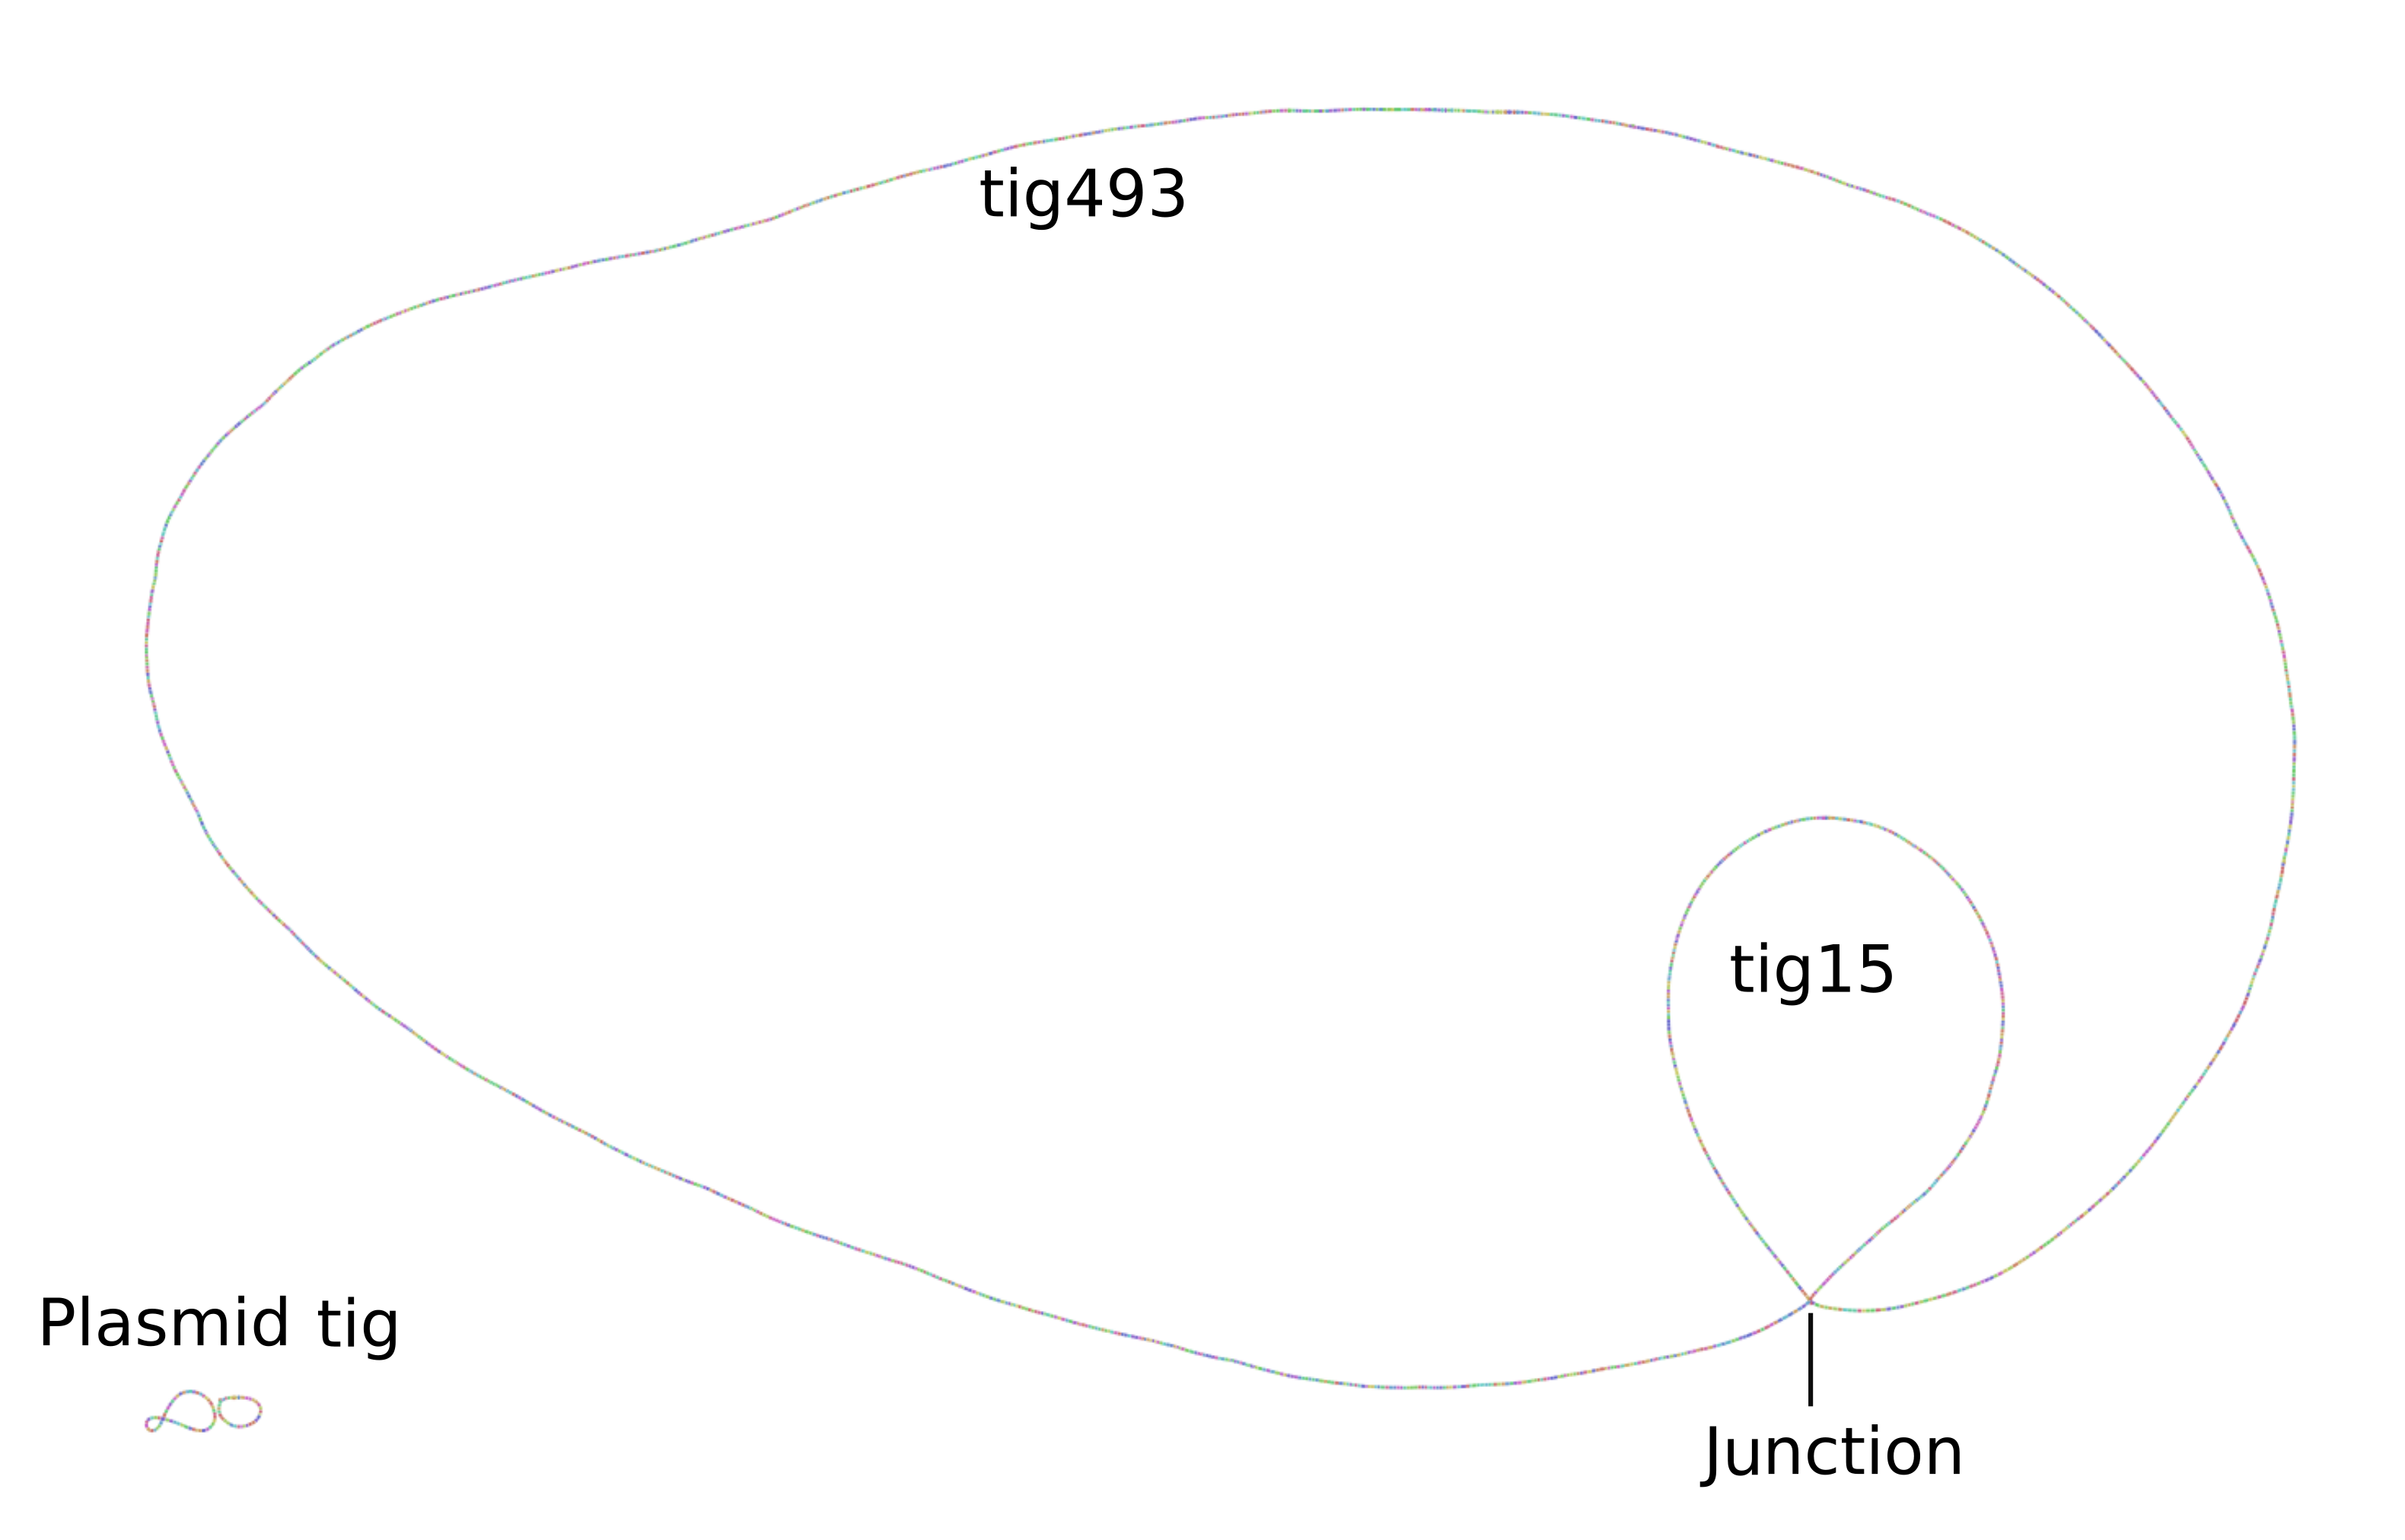
\includegraphics[width=\textwidth]{supplemental/knot/NCTC9078bog.png}
% \caption{Canu Best Overlap Graph of NCTC9078. We see two little components (bottom left): the two plasmid contigs reported in Table \ref{tb:nctc_dataset_assemblies}. The big component corresponds to the two main chromosomal contigs (tig493 and tig15). tig492 is found as a bubble in tig493. The junction  denotes a repetition: tig14 is at this junction.}
% \label{fg:appendix:bogNCTC9078}
% \end{figure}

\subsection*{NCTC12123}

\begin{figure}[!hb]

    \centerline{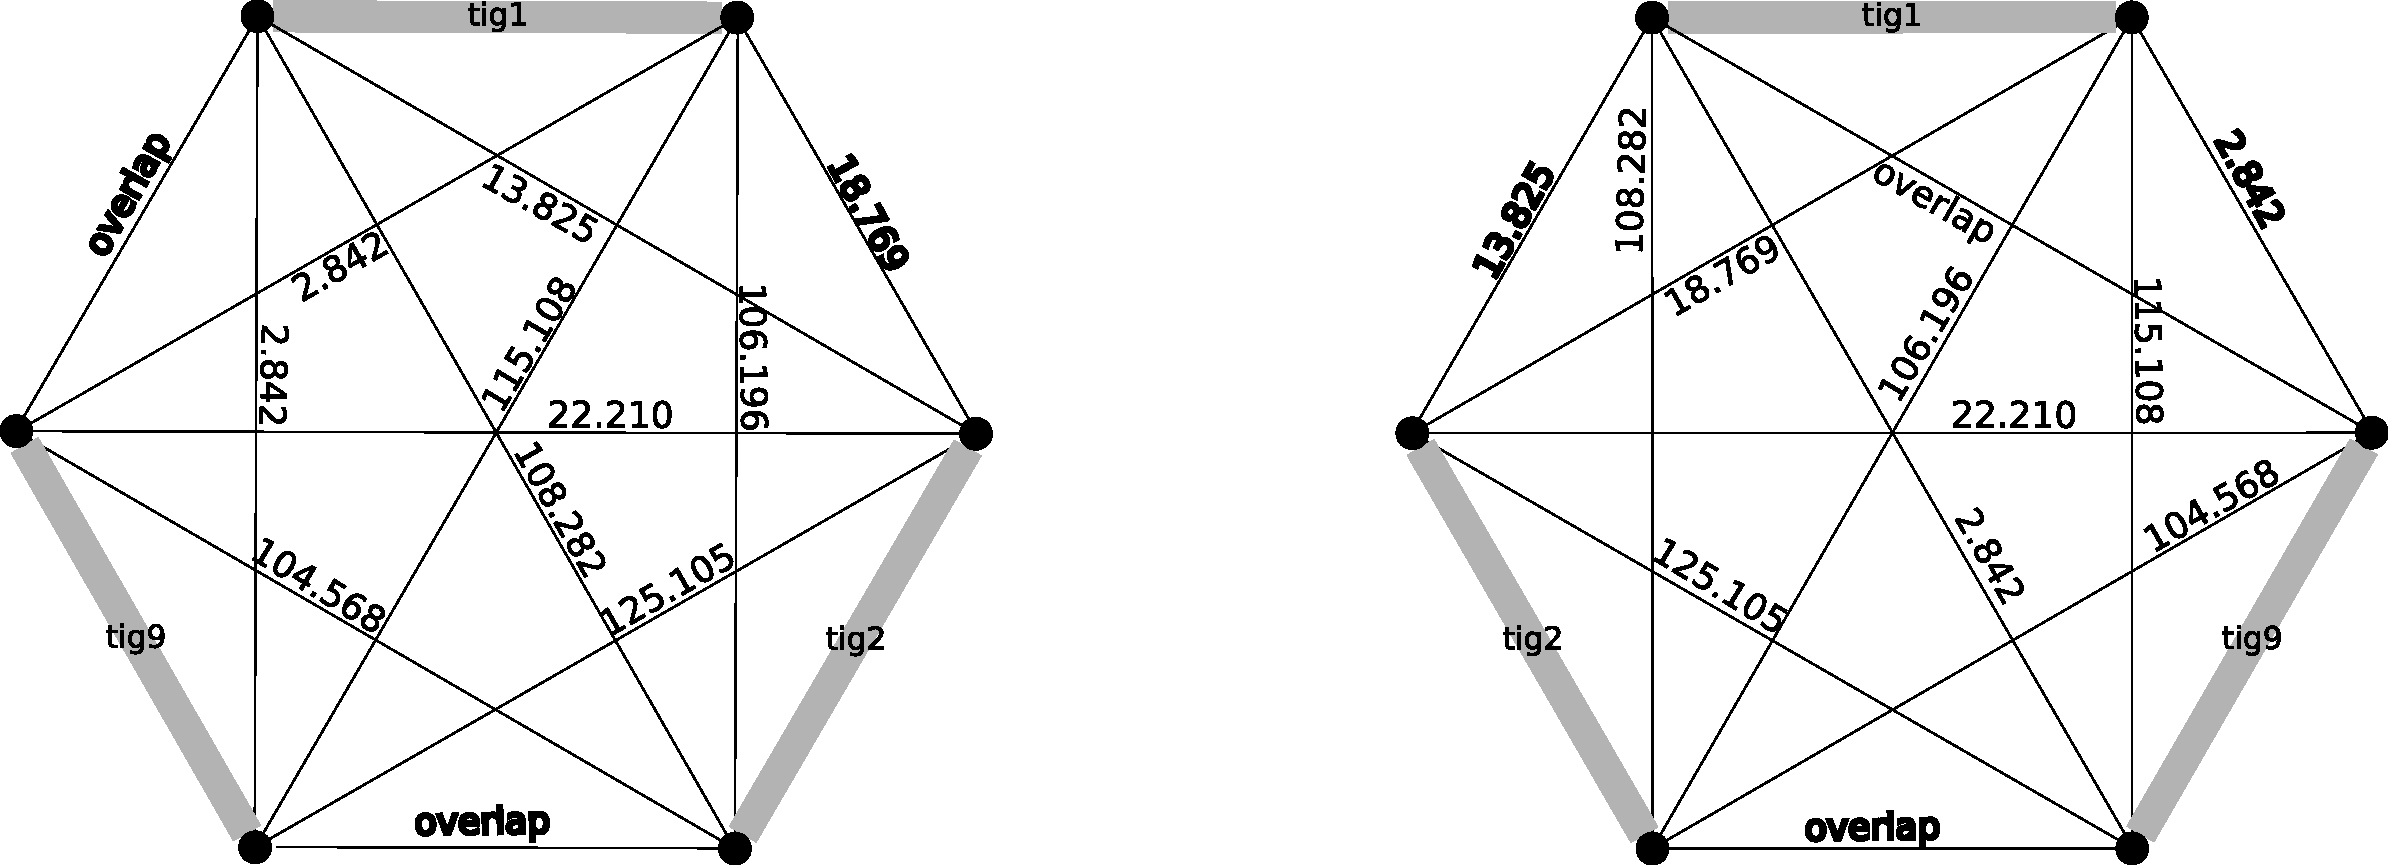
\includegraphics[width=\textwidth]{supplemental/knot/NCTC12123_possible_solution-crop.pdf}}
  %(a) NCTC12123 contigs mapped against NCTC reference for orderging. Paths from \canu (top dotted %edges) and \minimap (bottom dotted edges) are shown along with their number of reads as labels. Note that shortest paths in the \minimap SG from the left extremity of tig9 are searched manually because the read automatically selected did not have outgoing edges.  
%       
%        \jsv{je me demande vraiment si c'est utile ... qu'est-ce qui, dans le rapport, permet de voir cela immédiatement ?} \rc{Bonne question. On pourrait mettre ce qui concerne les overlaps en appendix dans la legende, qu'en dis-tu? }
%
    %In the \canu assembly,  tig1 and tig2 overlap over $\approx$8Kbp. tig2 and tig9 overlap over $\approx$6Kbp but we observe an intriguing drop of coverage in reads (both raw reads and those corrected by \canu) at the location of this overlap, 
    %That could explain why Canu has been unable to join those two contigs despite evidence of a path of overlapping reads unambiguously joining them. 
    %NCBI-Blast indicates that this overlap region matches a plasmid present in this species.
%
%
        %(b)
    \caption{
        Shortest paths in AAG. Both scenarii (paths that follow edges with bold label) use the edge of weight 7.178, the only remaining ambiguity concerns the order of tig1 against the pair tig2/tig9. 'overlap' indicate than our pipeline found an overlap between the contig extremities. The left scenario has a weight of 29.379 ($22.201 + 7.178$) while the right one has a weight of 30.736 ($17.209 + 7.178 + 6.349$).\ 
     }
     \label{fg:appendix:NCTC12123_solutions}
\end{figure}

~

\subsubsection*{NCTC5050}

\begin{figure}[!hb]

%\subfloat[]{
%    \centering
        {\small
    \ttfamily
    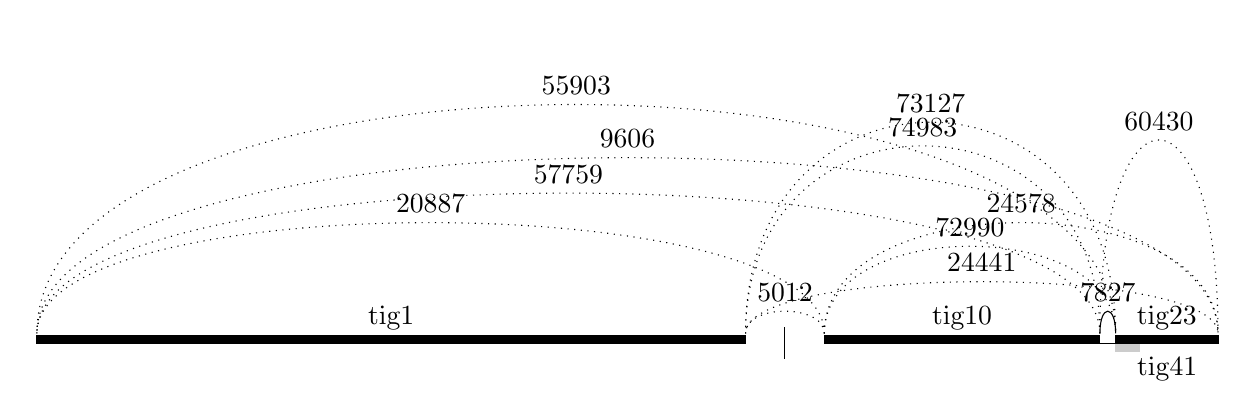
\begin{tikzpicture}
        \draw (0,0) node (1Left) {};
        \draw (9,0) node (1Right) {};
        
        \draw (10, 0) node (10Left) {};
        \draw (13.5, 0) node (10Right) {};
        
        \draw (13.7, 0) node (23Left) {};
        \draw (15, 0) node (23Right) {};
        
        \draw (13.7, 0) node (41Left) {};
        \draw (14, 0) node (41Right) {};
        
        % dessin des contigs
        \draw[fill] (1Left) ++ (0,0.1) rectangle node[above] {tig1} (1Right);
        \draw[fill] (10Left) ++ (0,0.1) rectangle node[above] {tig10} (10Right);
        \draw[fill] (23Left) ++ (0,0.1) rectangle node[above] {tig23} (23Right);
                
        % dessing des containments
        \draw[fill,color=black!20] (41Left) ++ (0,-0.1) rectangle node[below right, color=black] {tig41} (41Right);
        
        % liens canu qui respectent la reference NCTC
        \draw (10Right)
        .. controls +(up:5mm) and +(up:5mm) ..
        node[above] {7827} (23Left);
        
        % liens canu qui ne respectent pas la reference NCTC
        \draw[dotted] (10Left)
        .. controls +(up:16mm) and +(up:16mm) ..
        node[above] {72990} (23Left);
       
        \draw[dotted] (1Right)
        .. controls +(up:37mm) and +(up:37mm) ..
        node[above] {73127} (23Left);
       
        \draw[dotted] (1Left)
        .. controls +(up:40mm) and +(up:40mm) ..
        node[above] {55903} (23Left);
        
        \draw[dotted] (10Right)
        .. controls +(up:34mm) and +(up:34mm) ..
        node[above] {60430} (23Right);
        
        \draw[dotted] (10Left)
        .. controls +(up:20mm) and +(up:20mm) ..
        node[above] {24578} (23Right);
       
        \draw[dotted] (1Right)
        .. controls +(up:10mm) and +(up:10mm) ..
        node[above] {24441} (23Right);
       
        \draw[dotted] (1Left)
        .. controls +(up:31mm) and +(up:31mm) ..
        node[above] {9606} (23Right);
        
        \draw[dotted] (10Right)
        .. controls +(up:33mm) and +(up:33mm) ..
        node[above] {74983} (1Right);
        
        \draw[dotted] (10Left)
        .. controls +(up:20mm) and +(up:20mm) ..
        node[above] {20887} (1Left);
       
        \draw[dotted] (10Right)
        .. controls +(up:25mm) and +(up:25mm) ..
        node[above] {57759} (1Left);
       
        \draw[dotted] (10Left)
        .. controls +(up:5mm) and +(up:5mm) ..
        node[above] {5012} (1Right);
        
        % liens minimap qui respectent la reference NCTC
                % liens canu qui respectent la reference NCTC

        % dessin du génome (en dernier pour masquer)
        \draw (0,0) -- (9,0);
        \draw (9.5, -0.2) -- (9.5, 0.2);
        \draw (10,0) -- (15,0);
    \end{tikzpicture}}
%        \label{fg:appendix:NCTC5050_mapped_graph}
%}

%\centering\subfloat[]{
%    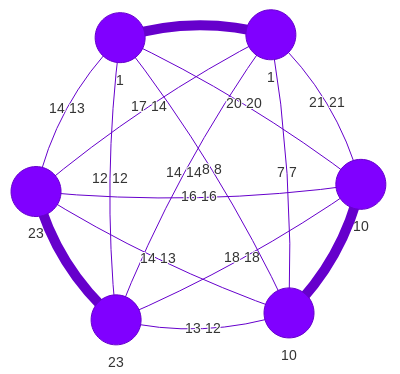
\includegraphics[width=0.3\textwidth]{supplemental/knot/contig_graph_NCTC5050-crop.png}
%    \label{fig:appendix:augmented_contig_graph}
%}

\caption{
NCTC5050 contigs mapped against NCTC reference for ordering. Paths are shown along with their number of bases as labels. The NCTC assembly consists of two contigs, hence the relative order of tig1 and tig10/tig23 cannot be inferred (vertical line in the figure). We observed that a portion of tig1 is inverted with respect to the NCTC assembly, with no impact on the path analysis as this putative misassembly does not involve an extremity of the contig.
%
%(b) NCTC5050 \minimap AAG generated during assembly report generation. We have 3 contig and all contig extremities are linked together, by a path found in the \minimap SG.
}
\label{fg:appendix:NCTC5050}
\end{figure}


\begin{figure}[!htbp]
    \centering
    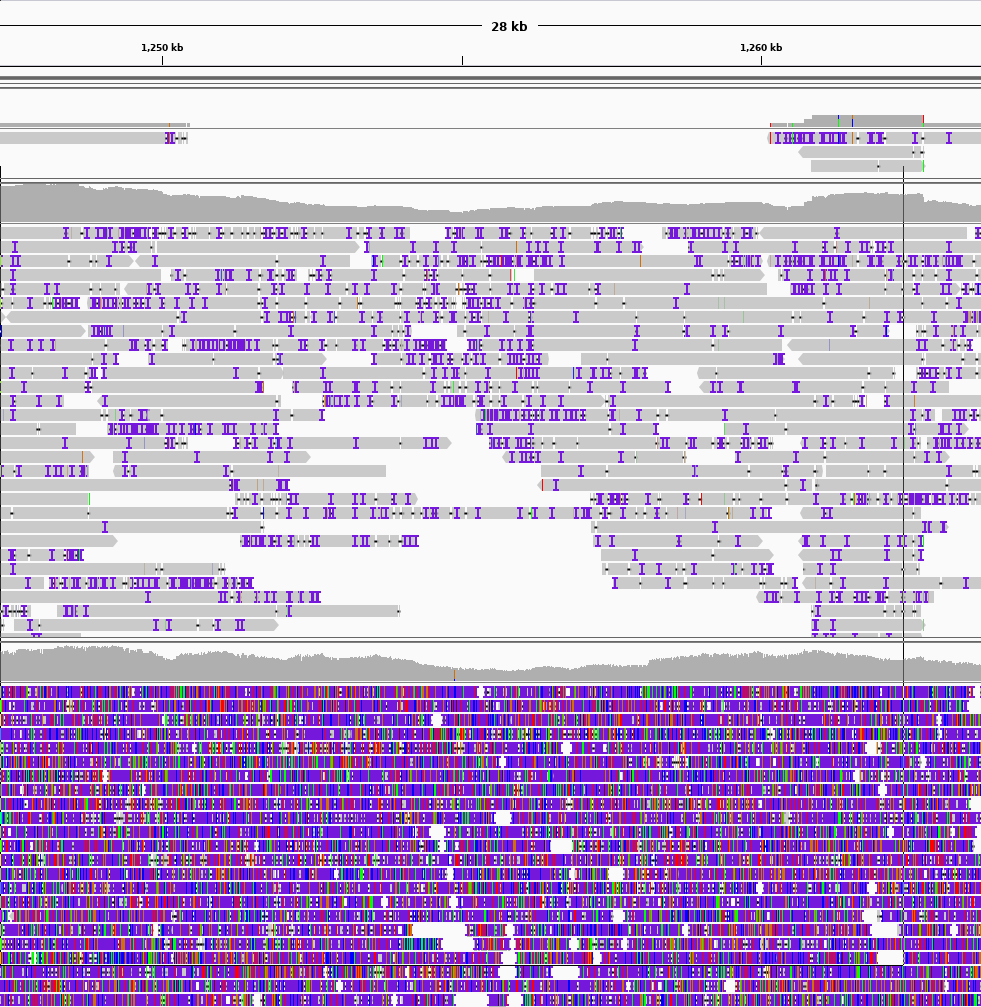
\includegraphics[width=\textwidth]{supplemental/knot/NCTC5050_tig10_tig23.png}
    \caption{IGV view of NCTC5050 mapping of \canu contig against NCTC contig, in junction between tig10 (first track at left) and tig23 (first track at right), tig41 are mapped on begin of tig23 in forward and reverse. The second track represent the mapping of \canu corrected read, the third track represent the raw reads. Above each this track we can observe the coverage curve and drop of this curve between the tig10 and tig23, for corrected read is around 50x coverage before junction, equal to 15x at minimal, and less than 40x after junction, this value are 90x, 25x and 40x for raw read. In addition we can observe more error in corrected read on this drop of coverage.}
    \label{fig:appendix:NCTC5050_tig10_tig23}
\end{figure}

\newpage

~

\section{YACRD: Yet Another Chimeric Read Detector}

\begin{figure}[!htbp]
    \centering
    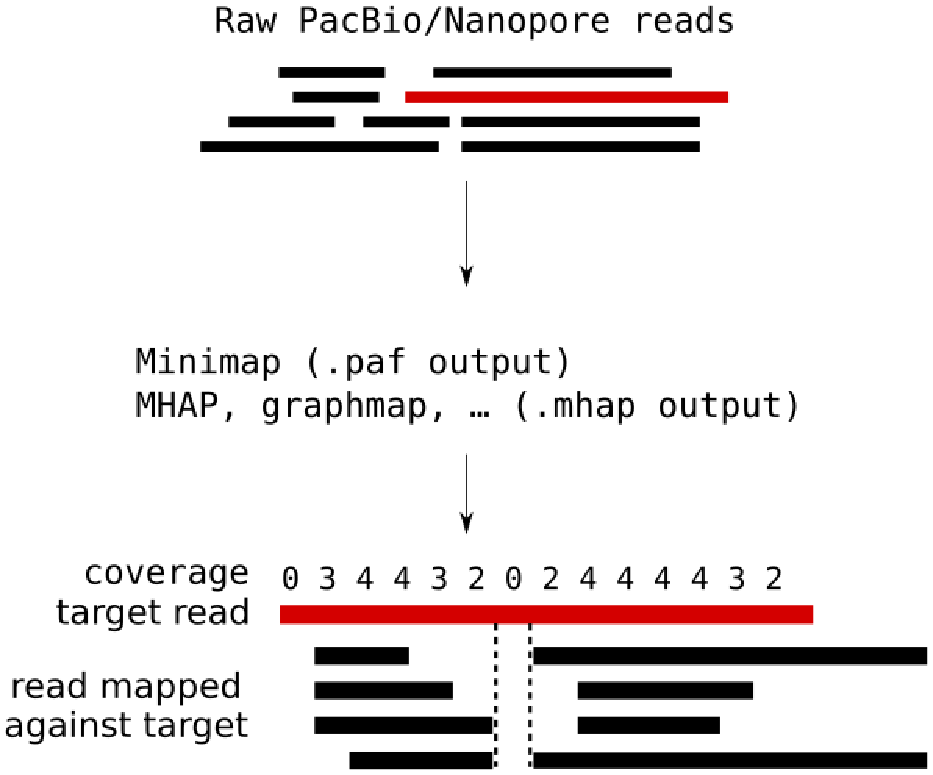
\includegraphics[width=0.6\textwidth]{supplemental/knot/yacrd.pdf}
    \caption{YACRD (manuscript in preparation) detects chimeric regions present in the read dataset. To detect such regions, YACRD takes as input the output of an overlapper (both PAF and MHAP format are accepted). For each read in the dataset, YACRD computes positional coverage values based on the overlaps with that read. If there is a drop of coverage, the corresponding read is marked as 'chimeric'.}
    \label{fig:appendix:yacrd}
\end{figure}

\end{document}